\documentclass[
	12pt,
	openright,
	oneside,
	a4paper,
	english,
	brazil
	]{abntex2}

% ---
% PACOTES BÁSICOS
% ---
\usepackage{lmodern}
\usepackage[T1]{fontenc}
\usepackage[utf8]{inputenc}
\usepackage{indentfirst}
\usepackage{color}
\usepackage{graphicx}
\usepackage{microtype}
\usepackage{amsmath}
\usepackage{listings}
\usepackage{xcolor}
\usepackage{url}
\usepackage{booktabs}
\usepackage{float}
\usepackage[alf]{abntex2cite}

% Configuração de código-fonte
\lstset{
  basicstyle=\footnotesize\ttfamily,
  breaklines=true,
  frame=single,
  captionpos=b,
  language=Python,
  keywordstyle=\color{blue},
  commentstyle=\color{gray},
  stringstyle=\color{red},
}

% ---
% INFORMAÇÕES DO TRABALHO
% ---
\titulo{FeelFrame: Sistema Web de Análise de Expressões Faciais e Emoções em Vídeos com Inteligência Artificial}
\autor{Leandro Diomar Gomes da Silva}
\local{Santo André}
\data{2026}
\orientador{Juliana Cristina Braga}
\instituicao{%
  UNIVERSIDADE FEDERAL DO ABC
  \par
  CMCC -- CENTRO DE MATEMÁTICA, COMPUTAÇÃO E COGNIÇÃO
  \par
  BACHARELADO EM CIÊNCIA DA COMPUTAÇÃO}
\tipotrabalho{Projeto de Graduação em Ciência da Computação}
\preambulo{Projeto de Graduação em Computação apresentado ao Bacharelado em Ciência da Computação da Universidade Federal do ABC, como requisito parcial para a obtenção do título de Bacharel.}

% ---
% CONFIGURAÇÕES DE APARÊNCIA E CAPA
% ---
\definecolor{blue}{RGB}{41,5,195}
\hypersetup{
    pdftitle={\@title},
    pdfauthor={\@author},
    pdfsubject={\imprimirpreambulo},
    colorlinks=true,
    linkcolor=black,
    citecolor=black,
    urlcolor=black
}

\renewcommand{\imprimircapa}{%
  \begin{capa}%
    \centering
    \vspace*{1cm}
    
\includegraphics[width=4cm]{imagens/Ufabc_logo.png} \\
    \vspace{0.5cm}
    {\ABNTEXchapterfont\large\imprimirinstituicao}
    
    \vspace*{\fill}
    
    {\ABNTEXchapterfont\large\imprimirautor}
    
    \vspace*{\fill}
    
    {\ABNTEXchapterfont\bfseries\LARGE\imprimirtitulo}
    
    \vspace*{\fill}
    
    {\large\imprimirlocal}
    \par
    {\large\imprimirdata}
    \vspace*{1cm}
  \end{capa}
}
% ---
% INÍCIO DO DOCUMENTO
% ---
\begin{document}

\selectlanguage{brazil}
\frenchspacing

% ----------------------------------------------------------
% ELEMENTOS PRÉ-TEXTUAIS
% ----------------------------------------------------------
\imprimircapa
\imprimirfolhaderosto

% --- Dedicatória ---
\begin{dedicatoria}
   \vspace*{\fill}
   \centering
   \noindent
   \textit{Dedico este trabalho aos meus pais, amigos e à minha namorada, que estiveram ao meu lado em cada etapa desta jornada e me ofereceram apoio incondicional ao longo de toda a trajetória acadêmica. Dedico também a todos que acreditam que a tecnologia e o conhecimento têm o poder de transformar vidas.}
   \vspace*{\fill}
\end{dedicatoria}

% --- Agradecimentos ---
\begin{agradecimentos}
Agradeço à minha orientadora pelo suporte, direcionamento e paciência ao longo do desenvolvimento deste projeto. Agradeço também à Universidade Federal do ABC pela formação de qualidade e pela infraestrutura disponibilizada.
Aos meus colegas e amigos Victor Cobo Figueiredo e Carlos Gabriell dos Anjos Quintino, meu sincero agradecimento por compartilharem comigo cada etapa desta longa e desafiadora jornada.
Por fim, aos meus pais e à minha namorada, por todo o suporte e apoio incondicional ao longo deste percurso — vocês foram essenciais.
\end{agradecimentos}

% --- Epígrafe ---
\begin{epigrafe}
    \vspace*{\fill}
	\begin{flushright}
		\textit{``Não é que eu seja tão inteligente, é que fico mais tempo com os problemas.''\\
		(Albert Einstein}
	\end{flushright}
\end{epigrafe}

% --- Resumo ---
\begin{resumo}
A compreensão automática de emoções humanas a partir de vídeos representa uma fronteira relevante da inteligência artificial com aplicações em educação, pesquisa de UX, saúde mental e marketing. Este trabalho apresenta o \textbf{FeelFrame}, um sistema web para análise automática de expressões faciais e estimativa de engajamento em vídeos. O sistema processa vídeos enviados pelo usuário, extrai frames, detecta rostos utilizando o detector YuNet, analisa emoções com a biblioteca DeepFace e rastreia pose de cabeça e direção do olhar com o MediaPipe FaceMesh. Os resultados são armazenados em banco de dados MongoDB e apresentados em uma interface estilo editor de vídeo, com uma linha do tempo multitrack de emoções. O back-end foi desenvolvido em Python com o framework FastAPI, oferecendo uma API RESTful com suporte a processamento assíncrono, Server-Sent Events para acompanhamento de progresso em tempo real e autenticação via JWT. O front-end foi construído com React (Vite), garantindo uma experiência responsiva e fluida. Os experimentos demonstraram a viabilidade do sistema na detecção das emoções básicas: Feliz, Triste, Surpreso, Medo e Neutro, além das dimensões comportamentais de concentração e engajamento.

\textbf{Palavras-chave}: Análise de Expressões Faciais. Reconhecimento de Emoções. Inteligência Artificial. Visão Computacional. DeepFace. MediaPipe. FastAPI. React.
\end{resumo}

% --- Abstract ---
\begin{resumo}[Abstract]
\begin{otherlanguage*}{english}
The automatic understanding of human emotions from videos represents a relevant frontier of artificial intelligence with applications in education, UX research, mental health, and marketing. This work presents \textbf{FeelFrame}, a web-based system for automatic facial expression analysis and engagement estimation in videos. The system processes user-submitted videos, extracts frames, detects faces using the YuNet detector, analyzes emotions with the DeepFace library, and tracks head pose and gaze direction with MediaPipe FaceMesh. Results are stored in a MongoDB database and presented through a video-editor-style interface featuring a multitrack emotion timeline. The back-end was developed in Python using the FastAPI framework, offering a RESTful API with asynchronous processing, Server-Sent Events for real-time progress tracking, and JWT-based authentication. The front-end was built with React (Vite), ensuring a responsive and fluid user experience. Experiments demonstrated the system's viability in detecting the basic emotions: Happy, Sad, Surprised, Fear, and Neutral, along with behavioral dimensions of concentration and engagement.

\vspace{\onelineskip}
\noindent
\textbf{Keywords}: Facial Expression Analysis. Emotion Recognition. Artificial Intelligence. Computer Vision. DeepFace. MediaPipe. FastAPI. React.
\end{otherlanguage*}
\end{resumo}

% --- Listas ---
\pdfbookmark[0]{\listfigurename}{lof}
\listoffigures*
\cleardoublepage

\pdfbookmark[0]{\listtablename}{lot}
\listoftables*
\cleardoublepage

% --- Sumário ---
\pdfbookmark[0]{\contentsname}{toc}
\tableofcontents*
\cleardoublepage

% ----------------------------------------------------------
% ELEMENTOS TEXTUAIS
% ----------------------------------------------------------
\textual

% ==========================================================
\chapter{INTRODUÇÃO}
% ==========================================================

O reconhecimento de emoções humanas é uma das capacidades mais complexas da cognição, e replicá-la computacionalmente tem sido um dos grandes desafios da inteligência artificial moderna. As expressões faciais são o canal mais rico e universal de comunicação emocional: estima-se que mais de 55\% da comunicação humana seja não-verbal, e o rosto representa a maior parte desse canal \cite{mehrabian1971silent}.

Com o avanço da produção de conteúdo educacional digital e de Jogos Educacionais Digitais (JEDs), surgiu a necessidade de ferramentas capazes de avaliar a eficácia desses materiais durante sua fase de concepção e testes empíricos. O FeelFrame foi idealizado para ser empregado na fase de avaliação pedagógica, antes do lançamento de uma tecnologia no mercado. Seu propósito não é o monitoramento contínuo de discentes em tempo real --- prática que esbarra em complexas questões éticas ---, mas atuar estritamente como um instrumento de teste, com o intuito de analisar o engajamento de objetos de aprendizagem (OAs), contribuindo assim para a avaliação de qualidade dos OAs existentes e para o projeto de OAs que ainda estão sendo desenvolvidos.

Este trabalho parte diretamente de uma pesquisa anterior realizada na Universidade Federal do ABC: o Trabalho de Conclusão de Curso de Nelson Nascimento \cite{nascimento2024nelson}, cujos resultados foram também publicados no Simpósio Brasileiro de Informática na Educação \cite{nascimento2024sbie}. Essa pesquisa original desenvolveu um algoritmo robusto capaz de detectar emoções faciais e estimar o nível de engajamento a partir de vídeos, combinando visão computacional e aprendizado profundo. O algoritmo original, embora cientificamente sólido, foi concebido para execução em ambiente local --- um script Python que exige instalação de dependências específicas e domínio técnico para operação --- sendo inacessível ao usuário final não especializado. O principal desafio deste PGC é, portanto, de engenharia de produto: transpor essa pesquisa acadêmica para o ambiente web, preservando e ampliando suas capacidades analíticas em uma plataforma acessível e escalável.

Neste contexto, o \textbf{FeelFrame} é proposto como um sistema web completo que automatiza o processo de análise de expressões faciais em vídeos gravados. O usuário faz o upload de um vídeo, o sistema processa cada frame, detecta o rosto, classifica as emoções, estima o engajamento e apresenta todos esses dados em uma linha do tempo interativa dentro de uma interface estilo editor de vídeo.

\section{PROBLEMA DE PESQUISA}

A análise manual de expressões faciais em vídeos é um processo trabalhoso, subjetivo e não escalável. As ferramentas comerciais existentes (como o iMotions e o Affectiva) têm custo elevado e não oferecem abertura técnica para customização. Ferramentas de código aberto, por sua vez, exigem conhecimento técnico avançado para configuração e não possuem interface amigável.

O problema central deste trabalho é: \textit{Como trabalhando baseado no algoritmo de detecção de emoções e engajamento desenvolvido por Nelson Nascimento  \cite{nascimento2024nelson} em um produto de software web acessível, escalável e utilizável por qualquer pessoa sem conhecimento técnico especializado, sem sacrificar o rigor analítico da pesquisa original?}

\section{OBJETIVOS}

\subsection{Objetivo Geral}

Desenvolver o sistema \textbf{FeelFrame}: uma aplicação web completa para análise automática de expressões faciais, classificação de emoções e estimativa de engajamento em vídeos, utilizando bibliotecas de visão computacional de código aberto. Com intuito de analisar o engajamento de objetos de aprendizagem, contribuindo assim para avaliação de qualidade dos Oas existentes e o para o projeto de OAs que ainda estão sendo desenvolvidos.com intuito de analisar o engajamento de objetos de aprendizagem, contribuindo assim para avaliação de qualidade dos Oas existentes e o para o projeto de OAs que ainda estão sendo desenvolvidos.

\subsection{Objetivos Específicos}

\begin{itemize}
    \item Classificar o nivel de engajamento dos estudantes;
    
    \item Implementar um pipeline de processamento de vídeo capaz de extrair frames, detectar rostos e classificar emoções;

    
    \item Desenvolver um back-end RESTful com suporte a processamento assíncrono e acompanhamento de progresso em tempo real via Server-Sent Events (SSE);
    \item Criar um front-end responsivo com interface estilo editor de vídeo e linha do tempo de emoções;
    \item Implementar um sistema de autenticação seguro com suporte a email/senha;
    \item Integrar armazenamento em nuvem (Firebase Storage) para persistência dos vídeos processados;
    \item Disponibilizar geração de relatórios em PDF com os resultados da análise;
    \item Avaliar a precisão e a viabilidade do sistema em cenários de uso real.
\end{itemize}

\section{JUSTIFICATIVA}

O FeelFrame se justifica em múltiplas frentes:

\textbf{Acadêmica}: Contribui para a pesquisa em reconhecimento afetivo computacional (\textit{affective computing}), área fundada por Rosalind Picard \cite{picard1997affective}, ao implementar um sistema integrado e funcional.

\textbf{Educacional}: O sistema atua como uma ferramenta de testes de usabilidade e avaliação pedagógica, permitindo entender como os objetos de aprendizagem e jogos educacionais podem engajar ou não o público-alvo a fim de ajudar na aprendizagem dos alunos. Isso é feito baseando-se em evidências emocionais e comportamentais extraídas de sessões de teste controladas, indicando em quais pontos exatos a tecnologia falha em manter o interesse.

\textbf{Técnica}: O trabalho demonstra a integração de tecnologias modernas (DeepFace, MediaPipe, FastAPI, React, MongoDB, Firebase) em um produto coeso e funcional.

\textbf{Continuidade de pesquisa}: O FeelFrame atua como elo entre a pesquisa científica do Prof. Nelson \cite{nascimento2024nelson} e a engenharia de software aplicada, demonstrando como resultados acadêmicos podem ser transpostos para produtos utilizáveis pela comunidade. Para entender como objetos de aprendizagem podem engajar ou não.

\section{DISCIPLINAS FORMADORAS DO PROJETO}

A construção do FeelFrame mobilizou conhecimentos adquiridos ao longo do curso de Bacharelado em Ciência da Computação da UFABC. A Tabela~\ref{tab:disciplinas} relaciona as principais disciplinas cursadas com as contribuições diretas que cada uma trouxe ao desenvolvimento do sistema.

\begin{table}[H]
\centering
\caption{Disciplinas do BCC/UFABC e sua contribuição ao FeelFrame}
\label{tab:disciplinas}
\resizebox{\textwidth}{!}{%
\begin{tabular}{|p{5.5cm}|p{3.5cm}|p{7.5cm}|}
\hline
\textbf{Disciplina} & \textbf{Código} & \textbf{Contribuição ao FeelFrame} \\ \hline

Inteligência Artificial & MCTA014-15 &
Fundamentos de aprendizado de máquina, redes neurais e classificadores que embasam o uso do DeepFace para reconhecimento de emoções a partir de CNNs pré-treinadas. \\ \hline

Programação Orientada a Objetos & MCTA018-13 &
Modelagem das entidades do sistema (usuário, vídeo, frame, marcador) com encapsulamento e separação de responsabilidades, viabilizando a arquitetura em camadas (\textit{routes / services / models}) do back-end FastAPI. \\ \hline

Engenharia de Software & MCTA033-15 &
Princípios de arquitetura de software, design de APIs RESTful, versionamento e boas práticas de desenvolvimento que guiaram a estruturação do projeto em módulos coesos e extensíveis. \\ \hline

Processamento de Linguagem Natural & MCZA017-13 &
Técnicas de processamento de dados não estruturados e pipelines de análise automatizada que influenciaram a concepção do pipeline de processamento de frames e geração de relatórios textuais. \\ \hline

Modelagem de Banco de Dados & MCCC012-23 &
Projeto dos esquemas das coleções MongoDB (\texttt{users}, \texttt{videos}, \texttt{frame\_analysis}, \texttt{markers}), definição de índices, estratégias de integridade referencial em nível de aplicação e consultas eficientes por \texttt{video\_id}. \\ \hline

Sistemas Distribuídos & MCTA025-13 &
Conceitos de processamento assíncrono, consistência eventual e comunicação entre serviços que fundamentaram o uso de \texttt{BackgroundTasks}, Server-Sent Events (SSE) e a integração com Firebase Storage como serviço externo de armazenamento. \\ \hline

Algoritmos e Estruturas de Dados II & MCTA002-17 &
Estruturas de dados eficientes para indexação temporal dos frames analisados e algoritmos de percurso usados na construção da linha do tempo multitrack de emoções exibida na interface. \\ \hline

Programação para Web & MCZA019-17 &
Desenvolvimento do front-end em React (Vite), implementação do contexto de autenticação com JWT no \textit{localStorage}, integração com a API via \textit{fetch} assíncrono e construção da interface estilo editor de vídeo com linha do tempo interativa. \\ \hline

\end{tabular}%
}
\fonte{O Autor (2026)}
\end{table}

\section{ORGANIZAÇÃO DO TEXTO}

Este documento está organizado da seguinte forma: o Capítulo \ref{cap:referencial} apresenta o referencial teórico sobre visão computacional, reconhecimento de expressões faciais e as tecnologias utilizadas; o Capítulo \ref{cap:revisao} revisa a literatura e os trabalhos correlatos; o Capítulo \ref{cap:desenvolvimento} descreve a arquitetura e o desenvolvimento do sistema; o Capítulo \ref{cap:metodologia} explica a metodologia de pesquisa e avaliação; o Capítulo \ref{cap:resultados} apresenta e discute os resultados obtidos; e o Capítulo \ref{cap:conclusao} traz as conclusões e trabalhos futuros.

% ==========================================================
\chapter{REFERENCIAL TEÓRICO}
\label{cap:referencial}
% ==========================================================

\section{Dinâmica das Emoções e Engajamento}

A compreensão do estado afetivo vai além do reconhecimento estático de expressões discretas, exigindo a análise da trajetória temporal dessas emoções. Compreender o engajamento de um indivíduo durante uma atividade pode contribuir significativamente para garantir que os objetivos da interação sejam plenamente atingidos. Em ambientes tradicionais e digitais, esse engajamento pode ser observado tanto por meio da linguagem corporal quanto pelas emoções faciais.

A determinação precisa do nível de envolvimento de um usuário tem se mostrado um desafio complexo, exigindo abordagens abrangentes. Modelos híbridos que combinam a coleta automática de expressões e posturas físicas com dados de autorrelatos (como pré e pós-questionários) oferecem um mapeamento mais robusto do perfil e das sensações experimentadas. A estruturação dessas avaliações baseia-se fortemente em pilares da psicologia e computação afetiva:
\begin{itemize}
    \item A utilização de bases como a Teoria das Seis Emoções Básicas e o Modelo Circumplexo de Russell;
    \item A estruturação de uma representação da dinâmica das emoções, focada na alternância contínua de estados afetivos;
    \item A percepção empírica de que o engajamento é essencialmente contextual e temporal;
    \item O entendimento de que o engajamento muitas vezes é menos proeminente ou explícito apenas na face do usuário;
    \item A constatação de que, antes de se desengajar completamente de um processo, o usuário transita por estados afetivos intermediários;
    \item A evidência de que o desengajamento ocorre de forma acentuada quando o indivíduo enfrenta dificuldades em manter o controle das ações ou interações propostas.
\end{itemize}

Dentro do escopo do FeelFrame, a fusão das métricas extraídas (como direção do olhar, abertura dos olhos e pose da cabeça) com a classificação afetiva cria as bases para a inferência dessa métrica complexa.

\section{Arquitetura de Software para Análise Contínua}

A eficácia de um sistema de visão computacional não depende exclusivamente da precisão de seus modelos, mas da infraestrutura tecnológica projetada para orquestrar o processamento. A manipulação de fluxos de vídeo e a execução paralela de algoritmos pesados de inferência requerem uma arquitetura reativa, escalável e de alto desempenho.

A integração dos detectores de face e classificadores de emoção demanda um \textit{back-end} capaz de gerenciar requisições assíncronas de forma otimizada, utilizando frameworks de alta performance como FastAPI. Simultaneamente, o volume de dados contínuos gerado pela análise \textit{frame a frame} --- contendo metadados de marcos faciais (\textit{landmarks}), poses de cabeça e intensidades emocionais --- requer um armazenamento ágil. Bancos de dados não relacionais e orientados a documentos, como o MongoDB ou Firebase, aderem perfeitamente a esse modelo, permitindo a ingestão rápida de séries temporais não rígidas.

Na ponta da interação, o consumo desses metadados processados deve ser traduzido em painéis visuais intuitivos. A construção de uma interface de usuário rica e componentizada, empregando bibliotecas modernas de \textit{front-end} como React, viabiliza a renderização de gráficos em tempo real, permitindo uma interpretação clara da dinâmica de atenção e das métricas emocionais geradas pelo sistema.

\section{Visão Computacional}

Visão computacional é o campo da inteligência artificial que busca fazer com que computadores interpretem e compreendam o conteúdo de imagens e vídeos digitais. Ela combina técnicas de processamento de imagem, aprendizado de máquina e geometria projetiva para extrair informações significativas de pixels \cite{szeliski2010computer}.

No contexto de análise facial, as principais tarefas de visão computacional são:
\begin{itemize}
    \item \textbf{Detecção de rosto}: localizar a região do rosto em uma imagem;
    \item \textbf{Alinhamento de marcos faciais} (\textit{landmark detection}): identificar pontos-chave como olhos, nariz, boca e contorno do rosto;
    \item \textbf{Reconhecimento de expressão}: classificar a expressão facial em categorias emocionais;
    \item \textbf{Estimativa de pose de cabeça}: determinar a orientação tridimensional da cabeça;
    \item \textbf{Estimativa de direção do olhar} (\textit{gaze estimation}): inferir para onde a pessoa está olhando.
\end{itemize}

\section{Teorias das Emoções Básicas}

A teoria mais influente sobre expressões faciais universais é a de Paul Ekman \cite{ekman1971constants}, que identificou seis emoções básicas com expressões faciais reconhecíveis independentemente de cultura: \textit{alegria, tristeza, surpresa, medo, raiva} e \textit{nojo}. Posteriormente, o \textit{Sistema de Codificação de Ações Faciais} (FACS -- \textit{Facial Action Coding System}) foi desenvolvido para descrever objetivamente os movimentos musculares do rosto em termos de \textit{Unidades de Ação} (AUs) \cite{ekman1978facial}.

O FeelFrame adota uma versão simplificada e mapeada dessas categorias, classificando as emoções em: \textbf{Feliz, Triste, Surpreso, Medo} e \textbf{Neutro}. As emoções de raiva e nojo são mapeadas para ``Triste'' por apresentarem perfis de expressão negativos similares em ambientes de vídeo.

\section{Aprendizado Profundo para Reconhecimento de Emoções}

O reconhecimento de expressões faciais evoluiu significativamente com o advento das Redes Neurais Convolucionais (CNNs). Antes disso, abordagens baseadas em SVM com descritores HOG ou LBP eram predominantes \cite{dalal2005histograms}. Com as CNNs, passou a ser possível aprender representações diretamente dos pixels com muito maior precisão.

O \textbf{DeepFace}, biblioteca utilizada neste trabalho, é um framework Python que encapsula múltiplos modelos pré-treinados de reconhecimento facial e análise de emoções, incluindo VGG-Face, Facenet, OpenFace e DeepFace \cite{serengil2020lightface}. Para análise de emoções, utiliza modelos treinados no conjunto de dados FER-2013, que contém aproximadamente 35.000 imagens de rostos rotuladas em sete categorias de emoção.

\section{MediaPipe FaceMesh}

O MediaPipe FaceMesh \cite{lugaresi2019mediapipe} é uma solução desenvolvida pelo Google para detecção de 468 marcos faciais em tempo real. Utiliza um pipeline de duas etapas: um detector de rosto leve baseado em BlazeFace, seguido por um modelo de regressão de marcos. Com \texttt{static\_image\_mode=True} (configuração adotada neste trabalho), funciona de forma stateless, processando cada frame de forma independente sem estado entre chamadas -- o que o torna seguro para uso em ambientes multi-thread.

O FaceMesh é utilizado no FeelFrame para três finalidades:
\begin{enumerate}
    \item Localizar e extrair a região do rosto para alimentar o DeepFace;
    \item Estimar a pose de cabeça (yaw, pitch, roll) via algoritmo PnP (\textit{Perspective-n-Point});
    \item Calcular a direção do olhar a partir da posição relativa da íris nos cantos dos olhos.
\end{enumerate}

\section{Detecção de Rosto com YuNet}

O YuNet \cite{wu2023yunet} é um detector de rostos leve e eficiente baseado em rede neural convolucional, distribuído como modelo ONNX e integrado ao OpenCVs. Apresenta excelente desempenho em rostos pequenos e parcialmente tampados, com baixíssima latência. No FeelFrame, o YuNet é utilizado como detector primário de rostos, com optando pelo uso do FaceMesh quando o YuNet não está disponível.

\section{Estimativa de Pose de Cabeça}

A pose de cabeça é estimada usando o método PnP (Perspective-n-Point) do OpenCV \cite{bradski2000opencv}, que resolve a correspondência entre pontos 3D conhecidos do modelo de face e seus equivalentes 2D detectados nos marcos do FaceMesh. Os ângulos de Euler (yaw, pitch, roll) são extraídos da matriz de rotação resultante. O sistema classifica a cabeça como voltada para: frente, esquerda, direita, cima ou baixo, com thresholds de 15 graus.

\section{Arquitetura de Software}

\subsection{FastAPI}

O FastAPI \cite{fastapi2019} é um framework web moderno para Python, construído sobre Starlette e Pydantic, que permite criar APIs RESTful de alto desempenho com tipagem estática e documentação automática (Swagger/OpenAPI). Sua capacidade nativa de suporte a funções assíncronas (\texttt{async/await}) o torna ideal para operações de I/O intensivo, como upload de arquivos e acesso a banco de dados.

\subsection{MongoDB}

O MongoDB é um banco de dados NoSQL orientado a documentos \cite{mongodb2021}, que armazena dados em formato BSON (Binary JSON). Sua estrutura schema-free é adequada para o FeelFrame, pois os documentos de análise de frame têm estrutura variável e o volume de dados cresce rapidamente com o processamento de vídeos.

\subsection{Firebase Storage}

O Firebase Storage \cite{firebase2023} é um serviço de armazenamento de objetos na nuvem do Google, integrado ao Firebase Authentication. No FeelFrame, é utilizado para armazenar os vídeos originais e processados, disponibilizando URLs públicas para acesso direto pelo front-end.

\subsection{React e Vite}

O React \cite{react2023} é uma biblioteca JavaScript para construção de interfaces de usuário baseadas em componentes reativos. O Vite \cite{vite2023} é um bundler moderno que oferece um servidor de desenvolvimento ultrarrápido com Hot Module Replacement (HMR). Juntos, formam uma base sólida para SPAs (Single Page Applications) modernas.

\subsection{JWT -- JSON Web Tokens}

A autenticação no FeelFrame utiliza JWT \cite{jones2015json}, um padrão aberto (RFC 7519) para criação de tokens de acesso compactos e autocontidos. O token carrega o identificador do usuário e é assinado com uma chave secreta usando o algoritmo HMAC-SHA256. O tempo de expiração padrão é de 7 dias.

\subsection{Modelo Teórico de Engajamento}
\label{sec:modelo_engajamento}

O FeelFrame fundamenta-se no modelo teórico e computacional de detecção de engajamento, alinhado à pesquisa de Nascimento Junior \cite{nascimento2024nelson}, que integra conceitos da psicologia educacional e da computação afetiva para avaliar a interação do usuário com objetos de aprendizagem. Diferente de abordagens focadas apenas no desempenho de classificadores, este modelo compreende o engajamento como uma emoção complexa composta por dimensões integradas.

A dimensão comportamental é mensurada pelo nível de atenção, extraído através da pose da cabeça e da direção do olhar. A dimensão emocional baseia-se nas emoções básicas universais de Ekman \cite{ekman1971constants}, que são mapeadas no Modelo Circunflexo de Russell (1980), categorizando os estados afetivos nos eixos de valência (prazer versus desprazer) e ativação (energia). A partir da combinação de atributos observacionais (pose da cabeça, piscagem, direção do olhar e expressão facial), o modelo utiliza regras de decisão para classificar o estado do estudante em níveis distintos durante o uso da tecnologia:

\begin{itemize}
    \item \textbf{Fluxo (Flow)}: Representa o estado de alto engajamento, caracterizado por imersão total e satisfação durante uma atividade desafiadora \cite{csikszentmihalyi1990flow}. Ocorre quando há foco direcional (cabeça e olhos voltados para a tela) combinado com emoções de alta valência e ativação (feliz, surpreso) ou atenção neutra;
    \item \textbf{Engajado}: O usuário mantém o foco comportamental e a ativação fisiológica na tarefa, mesmo manifestando emoções de valência negativa (como raiva ou medo). Isso sinaliza um envolvimento cognitivo reativo com o jogo ou OA, indicando, por exemplo, superação de desafios ou frustração produtiva;
    \item \textbf{Desengajado}: Caracterizado por comportamentos de retirada de atenção, como olhos fechados ou desvio constante do olhar, independentemente da emoção expressa. Indica estados de baixa ativação, apatia ou tédio, sinalizando pontos onde o design educacional falhou em reter o usuário.
\end{itemize}

A utilização deste referencial no módulo de relatórios do FeelFrame permite que educadores e desenvolvedores identifiquem com precisão os instantes em que o fluxo ocorre ou é quebrado, servindo como base empírica para o refinamento do design de tecnologias educacionais.

\subsection{UMAP -- Redução de Dimensionalidade}

O UMAP (\textit{Uniform Manifold Approximation and Projection}) \cite{mcinnes2018umap} é um algoritmo avançado que reduz a complexidade dos dados de forma mais eficiente que o t-SNE. No FeelFrame, ele está implementado no \texttt{RelatorioService} para projetar as sete \textit{features} contínuas de cada frame (pose de cabeça, olhar e confiança de emoção) em espaços 2D e 3D, agrupando visualmente comportamentos semelhantes e permitindo, em tese, identificar rapidamente padrões e \textit{clusters} de engajamento no vídeo. Na versão atual do sistema, essa etapa está implementada como método isolado mas ainda não é chamada automaticamente durante a geração do relatório em PDF -- os detalhes dessa integração pendente são discutidos na Seção~\ref{sec:graficos_relatorio}.

% ==========================================================
\chapter{REVISÃO DE LITERATURA}
\label{cap:revisao}
% ==========================================================

\section{Estado da Arte em Reconhecimento de Emoções}

O reconhecimento de emoções a partir de expressões faciais tem sido amplamente estudado na última década. As abordagens modernas baseiam-se predominantemente em redes neurais profundas treinadas em grandes conjuntos de dados rotulados.

\textbf{AffectNet} \cite{mollahosseini2017affectnet} é um dos maiores conjuntos de dados de expressões faciais, com mais de um milhão de imagens coletadas da internet e anotadas com 11 categorias de expressões. Modelos treinados nesse conjunto atingem acurácia superior a 60\% na validação, refletindo a dificuldade inerente do problema.

\textbf{FER-2013} \cite{goodfellow2013challenges} é outro conjunto de dados amplamente utilizado, com 35.887 imagens de rostos em 48x48 pixels, classificadas em sete emoções. É o conjunto base dos modelos de emoção do DeepFace.

\textbf{Affectiva} \cite{mcduff2016affdex} é uma empresa pioneira em análise de emoções, oferecendo o SDK Affdex que analisa microexpressões em tempo real. Seus modelos são proprietários e não estão disponíveis para uso livre.

\textbf{OpenFace} \cite{baltrusaitis2018openface} é uma ferramenta de código aberto para análise facial que extrai AUs, pose de cabeça e direção do olhar. Diferentemente do FeelFrame, não classifica emoções diretamente, mas fornece dados brutos de AUs que podem ser mapeados para emoções.

\textbf{py-feat} \cite{cheong2023py} é uma biblioteca Python recente que unifica detecção de rosto, marcos faciais, AUs e emoções em uma única API. Mais completa que o DeepFace em termos de AUs, mas com maior overhead computacional.

\section{Sistemas de Análise de Engajamento}

O conceito de \textit{engajamento} em contextos educacionais tem sido explorado por múltiplos trabalhos. \cite{whitehill2014faces} propõe um framework para predição automática de engajamento de estudantes a partir de expressões faciais, usando SVMs com features de AUs. \cite{kaur2018prediction} avalia o engajamento de estudantes em cursos online usando combinação de expressão facial e direção do olhar.

O FeelFrame adota uma abordagem heurística para estimativa de engajamento, combinando três dimensões:
\begin{enumerate}
    \item \textbf{Dimensão comportamental}: derivada da pose de cabeça e direção do olhar (Concentrado / Distraído);
    \item \textbf{Valência emocional}: pontuação baseada na emoção detectada (positivas aumentam o score, negativas diminuem);
    \item \textbf{Estado de fluxo}: detectado quando o sujeito está concentrado e em estado emocional positivo \cite{csikszentmihalyi1990flow}.
\end{enumerate}

\section{Trabalho de Base: Nelson Nascimento Junior (2024)}
\label{sec:nelson}

O presente sistema tem sua origem direta no trabalho de Nelson Nascimento  \cite{nascimento2024nelson}, publicado no SBIE 2024 juntamente com a Profa Juliana Braga
\cite{nascimento2024sbie}. O algoritmo original combina o detector YuNet para localização de rostos, o MediaPipe FaceMesh para estimativa de pose de cabeça e direção do olhar, e o DeepFace para classificação de emoções --- exatamente o mesmo núcleo tecnológico adotado pelo FeelFrame.

A principal contribuição do presente PGC em relação ao trabalho original não reside na substituição ou reformulação do algoritmo de visão computacional, mas na sua \textbf{engenharia de produto}: a criação de uma arquitetura cliente-servidor completa, de uma API RESTful com autenticação e controle multi-usuário, e de uma interface web com linha do tempo interativa, funcionalidades de edição em lote e geração de relatórios. A Tabela~\ref{tab:diferencas} sintetiza as diferenças técnicas entre os dois sistemas.

\begin{table}[H]
\centering
\caption{Diferenças entre o algoritmo original \cite{nascimento2024nelson} e o FeelFrame}
\label{tab:diferencas}
\resizebox{\textwidth}{!}{%
\begin{tabular}{|c|c|c|}
\hline
\textbf{Aspecto}           & \textbf{Algoritmo Original}   & \textbf{FeelFrame}                           \\ \hline
Ambiente de execução       & Script Python local           & Aplicação web (FastAPI + React)            \\ \hline
Interface do usuário       & Terminal / arquivo de saída   & Interface gráfica responsiva               \\ \hline
Processamento              & Síncrono, bloqueante          & Assíncrono, BackgroundTasks + SSE          \\ \hline
Persistência               & Arquivos locais               & MongoDB + Firebase Storage                 \\ \hline
Edição de dados            & Não disponível                & Bulk update e marcadores interativos       \\ \hline
Relatório                  & Saída textual / CSV           & PDF com gráficos Plotly e análise detalhada\\ \hline
Dataset de calibração      & Base de controle original     & Base de dados externa para generalização   \\ \hline
\end{tabular}%
}
\fonte{O Autor (2026)}
\end{table}

A escolha de uma base de dados externa para calibração do modelo de emoção visou testar a capacidade de generalização do sistema em diferentes contextos de iluminação, câmera e diversidade demográfica, conforme discutido na Seção~\ref{sec:resultados_comparacao}.

\section{Ferramentas Similares}

A Tabela \ref{tab:comparativo} apresenta uma comparação entre o FeelFrame e ferramentas similares disponíveis no mercado e na academia.

\begin{table}[H]
\centering
\caption{Comparativo entre sistemas de análise emocional de vídeo}
\label{tab:comparativo}
\resizebox{\textwidth}{!}{%
\begin{tabular}{|c|c|c|c|c|c|}
\hline
\textbf{Sistema} & \textbf{Open Source} & \textbf{Web-based} & \textbf{Linha do Tempo} & \textbf{Edição} & \textbf{Custo} \\ \hline
FeelFrame                  & Sim & Sim & Sim & Sim & Gratuito  \\ \hline
Nascimento Jr. (2024)      & Sim & Não & Não & Não & Gratuito  \\ \hline
iMotions                   & Não & Não & Sim & Parcial & Alto      \\ \hline
Affectiva SDK              & Não & Parcial & Não & Não & Comercial \\ \hline
OpenFace                   & Sim & Não & Não & Não & Gratuito  \\ \hline
py-feat                    & Sim & Não & Não & Não & Gratuito  \\ \hline
\end{tabular}%
}
\fonte{O Autor (2026)}
\end{table}

% ==========================================================
\chapter{DESENVOLVIMENTO DO SISTEMA}
\label{cap:desenvolvimento}
% ==========================================================

\section{Visão Geral da Arquitetura}

O FeelFrame segue a arquitetura \textit{cliente-servidor}, composta por três camadas principais:

\begin{enumerate}
    \item \textbf{Front-end}: SPA React que oferece a interface do usuário -- login, upload de vídeos, visualização da análise e geração de relatórios;
    \item \textbf{Back-end}: API RESTful em FastAPI responsável pelo processamento dos vídeos, persistência dos dados e autenticação;
    \item \textbf{Infraestrutura}: MongoDB como banco de dados, Firebase Storage para armazenamento de vídeos.
\end{enumerate}

A Figura \ref{fig:arquitetura} ilustra a arquitetura geral do sistema.

\begin{figure}[H]
\centering
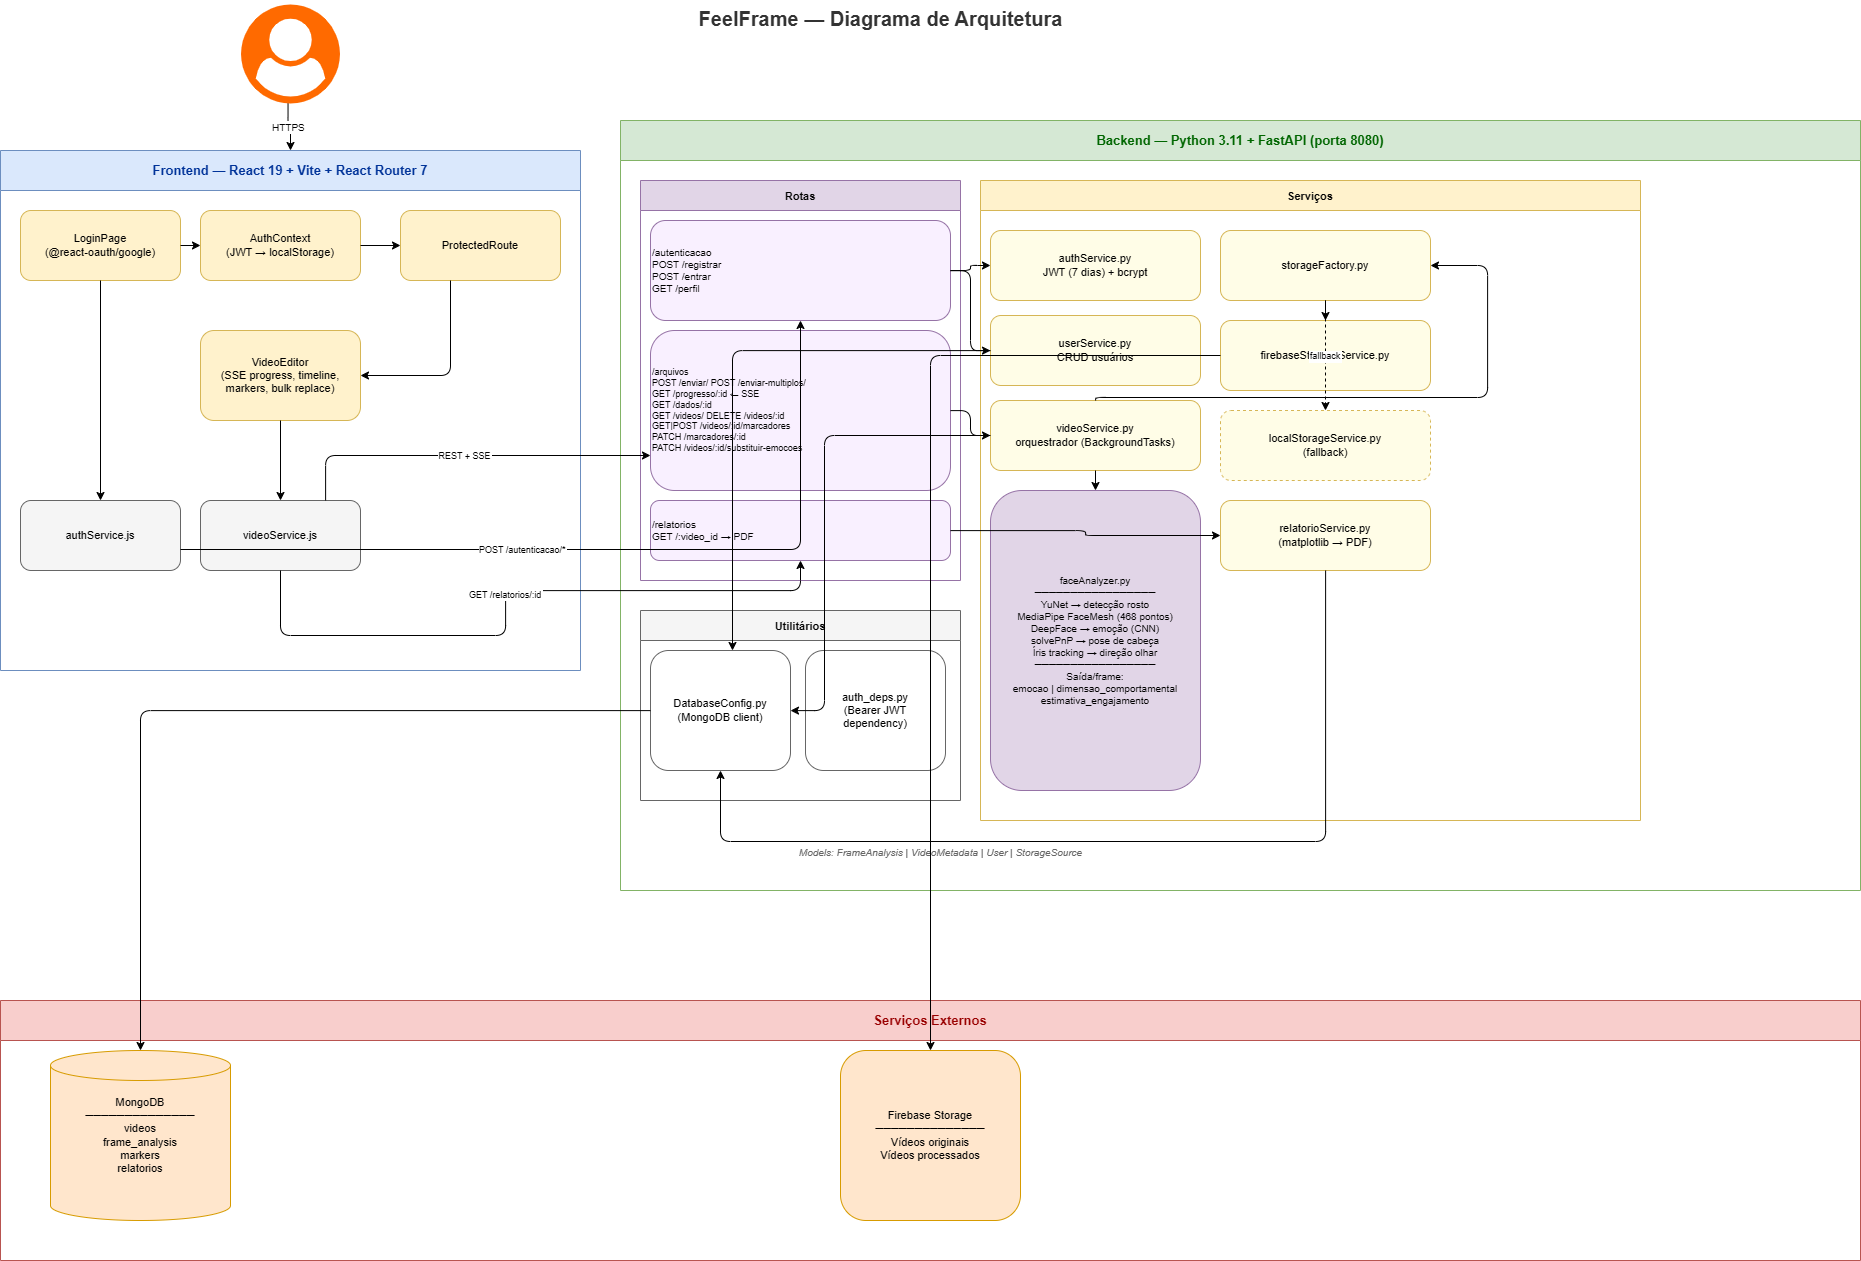
\includegraphics[width=\textwidth]{imagens/arquitetura.png}
\caption{Arquitetura geral do sistema FeelFrame}
\label{fig:arquitetura}
\fonte{O Autor (2025)}
\end{figure}

\section{Pipeline de Processamento de Vídeo}

O pipeline de processamento é o núcleo do FeelFrame. Ao receber um vídeo, o sistema executa as seguintes etapas:

\begin{enumerate}
    \item \textbf{Recebimento e registro}: O vídeo é recebido via upload HTTP, registrado no MongoDB com status \texttt{pending} e enviado para processamento assíncrono em background (FastAPI \texttt{BackgroundTasks});
    \item \textbf{Extração de frames}: O OpenCV percorre o vídeo frame a frame. A variável \texttt{frame\_analysis\_skip\_rate} controla quantos frames são analisados; na implementação atual, todos os frames são analisados (\texttt{skip\_rate=1}), maximizando a precisão temporal da linha do tempo de emoções ao custo de maior tempo de processamento;
    \item \textbf{Detecção de rosto e recorte fixo}: O YuNet detecta o rosto no \textbf{primeiro frame} do vídeo e o rect de recorte resultante (\textit{fixed\_crop\_rect}) é reutilizado em todos os frames subsequentes. Essa estratégia garante consistência espacial da análise e reduz o overhead de detecção por frame. Para o vídeo de saída, é gerado um recorte ampliado que inclui tronco superior e ombros; para a análise pelo DeepFace, é gerado um recorte em close do rosto, maximizando a qualidade de detecção de emoções. Se nenhum rosto for detectado no primeiro frame, frames pretos são gerados no vídeo de saída;
    \item \textbf{Análise de marcos}: O FaceMesh detecta os 468 marcos faciais e calcula pose de cabeça e direção do olhar;
    \item \textbf{Classificação de emoção}: A região do rosto é passada para o DeepFace, que retorna scores de probabilidade para cada categoria de emoção;
    \item \textbf{Cálculo de engajamento}: Com base na emoção, pose e olhar, é calculada a dimensão comportamental e a estimativa de engajamento;
    \item \textbf{Persistência em lote}: Os resultados de \texttt{FrameAnalysis} são acumulados em memória e persistidos em lote na coleção \texttt{frame\_analysis} do MongoDB a cada 150 frames (\textit{batch insert}), reduzindo o número de operações de I/O em banco de dados e o overhead de rede sem comprometer a integridade dos dados;
    \item \textbf{Armazenamento de vídeo}: O vídeo original e o vídeo processado (com quadro fixo de rosto) são enviados para o Firebase Storage;
    \item \textbf{Conclusão}: O documento do vídeo no MongoDB é atualizado para status \texttt{success} com as URLs dos vídeos armazenados.
\end{enumerate}

\section{Módulo de Análise Facial (FaceAnalyzer)}

O \texttt{FaceAnalyzer} é a classe central do pipeline, responsável pela análise de cada frame. Implementado com atenção a \textit{thread-safety}, utiliza \texttt{threading.Lock()} para proteger os históricos de emoções, pose e olhar compartilhados entre threads.

\subsection{Detecção de Emoção}

A detecção de emoção é realizada pelo DeepFace com \texttt{enforce\_detection=False} e \texttt{detector\_backend='skip'}, para que o rosto já recortado seja analisado diretamente. Três regiões do rosto são analisadas independentemente (face completa, região dos olhos, região da boca) e a que retorna maior confiança é utilizada. O mapeamento de emoções é:

\begin{table}[H]
\centering
\caption{Mapeamento de emoções DeepFace para categorias FeelFrame}
\label{tab:emocoes}
\begin{tabular}{|l|l|}
\hline
\textbf{Emoção DeepFace} & \textbf{Categoria FeelFrame} \\ \hline
happy                     & Feliz                        \\ \hline
sad                       & Triste                       \\ \hline
neutral                   & Neutro                       \\ \hline
surprise                  & Surpreso                     \\ \hline
fear                      & Medo                         \\ \hline
angry                     & Triste                       \\ \hline
disgust                   & Triste                       \\ \hline
\end{tabular}
\fonte{O Autor (2025)}
\end{table}

Correções heurísticas são aplicadas para reduzir falsos positivos de ``Triste'': se o score de tristeza/raiva/nojo é baixo (< 20), a emoção é reclassificada como Neutro.

\subsection{Estimativa de Pose de Cabeça}

A pose de cabeça é estimada com o algoritmo \texttt{cv.solvePnP}, usando 6 marcos faciais específicos (ponta do nariz, queixo, cantos dos olhos e boca) como pontos 2D e seu equivalente em um modelo 3D genérico do rosto humano. Os ângulos de yaw (rotação horizontal), pitch (rotação vertical) e roll (rotação axial) são extraídos da matriz de rotação.

\subsection{Estimativa de Direção do Olhar}

A direção do olhar é calculada pela posição relativa do centro da íris (estimada como centroide dos marcos 469-472 para o olho direito e 474-477 para o esquerdo) em relação aos cantos interno e externo dos olhos. O ratio horizontal ($r_h$) é definido como:

\begin{equation}
r_h = \frac{x_{\text{íris}} - x_{\text{canto externo}}}{|x_{\text{canto interno}} - x_{\text{canto externo}}|}
\end{equation}

Valores de $r_h < 0,40$ indicam olhar para a esquerda; $r_h > 0,60$, para a direita; intermediários, para o centro.

\subsection{Detecção de Olhos Fechados (EAR)}

O \textit{Eye Aspect Ratio} (EAR) é calculado independentemente para cada olho a partir dos marcos do FaceMesh, como a razão entre a distância vertical das pálpebras e a distância horizontal dos cantos:

\begin{equation}
\text{EAR} = \frac{\|p_{\text{top}} - p_{\text{bottom}}\|}{\|p_{\text{outer}} - p_{\text{inner}}\|}
\end{equation}

O EAR médio dos dois olhos é comparado ao threshold \texttt{OLHOS\_FECHADOS\_THRESHOLD=0{,}2}. Quando o valor cai abaixo desse limiar, o sistema classifica o estado comportamental do frame como \texttt{INDEFINIDO\_DISTRAIDO}, independentemente da pose de cabeça e da direção do olhar, pois olhos fechados indicam impossibilidade de avaliação de atenção visual e podem sinalizar sonolência ou distração profunda.

\subsection{Cálculo de Engajamento}

O engajamento é calculado por um sistema de pontuação:

\begin{equation}
\text{score} = \text{score\_dimensao} + \text{score\_emocao} \times \min\left(\frac{\text{confiança}}{0,5}, 1\right)
\end{equation}

Onde \texttt{score\_dimensao} varia de 5 (Distraído) a 70 (Concentrado), e \texttt{score\_emocao} varia de -10 (Triste/Medo) a +40 (Feliz). A classificação final é:
\begin{itemize}
    \item \textbf{Altamente Engajado}: score $\geq$ 80 ou estado de fluxo detectado;
    \item \textbf{Engajado}: score $\in$ [55, 80);
    \item \textbf{Desengajado}: score $\in$ [30, 55);
    \item \textbf{Altamente Desengajado}: score < 30.
\end{itemize}

\section{Calibração e Ajustes do Espectro Emocional}
\label{sec:calibracao_espectro}

O algoritmo original de Nascimento Junior \cite{nascimento2024nelson} não foi concebido como uma fórmula fixa e imutável, mas como um conjunto de regras heurísticas calibradas empiricamente sobre uma base de vídeos de controle, com pesos e limiares passíveis de ajuste conforme o domínio de aplicação e o perfil dos sujeitos analisados. O FeelFrame herda essa mesma filosofia: em vez de embutir um classificador único e monolítico, o \texttt{FaceAnalyzer} expõe um conjunto de constantes de calibração que determinam como sinais brutos de visão computacional (emoção, pose de cabeça, olhar, abertura dos olhos) são traduzidos em categorias discretas de engajamento. Essa característica é central para a continuidade científica do trabalho, pois permite que futuros pesquisadores recalibrem o sistema sem alterar sua arquitetura.

\subsection{Parâmetros Ajustáveis Identificados}

A Tabela~\ref{tab:calibracao} sintetiza os principais parâmetros de calibração do espectro emocional presentes na implementação atual, seus valores padrão e o efeito de sua variação.

\begin{table}[H]
\centering
\caption{Parâmetros de calibração do espectro emocional e de engajamento}
\label{tab:calibracao}
\resizebox{\textwidth}{!}{%
\begin{tabular}{|l|l|p{7.5cm}|}
\hline
\textbf{Parâmetro} & \textbf{Valor padrão} & \textbf{Efeito de ajuste} \\ \hline
\texttt{SAD\_TO\_NEUTRAL\_THRESHOLD} & 20 & Eleva ou reduz a sensibilidade da correção heurística de falsos positivos de ``Triste''/raiva/nojo; valores mais altos reclassificam mais frames ambíguos como Neutro \\ \hline
\texttt{SECOND\_EMOTION\_THRESHOLD} & 15,0 & Define a partir de qual diferença de score uma emoção secundária passa a ser considerada relevante na análise, afetando a granularidade de estados afetivos mistos \\ \hline
\texttt{OLHOS\_FECHADOS\_THRESHOLD} (EAR) & 0,2 & Sensibilidade da detecção de olhos fechados; valores menores toleram mais piscadas antes de classificar o frame como \texttt{INDEFINIDO\_DISTRAIDO} \\ \hline
Pesos de \texttt{score\_emocao} & Feliz +40, Surpreso +30, Neutro +20, Triste/Medo −10 & Determinam o peso de cada categoria emocional na pontuação final de engajamento; alterá-los desloca a fronteira entre estados considerados positivos e negativos \\ \hline
Pesos de \texttt{score\_dimensao} & Concentrado 70, Indefinido/Concentrado 55, Indefinido/Distraído 30, Distraído 5 & Determinam o peso da dimensão comportamental (pose/olhar) frente à dimensão emocional na composição do score final \\ \hline
Limiar de estado de fluxo & confiança $\geq$ 0,35 & Controla a facilidade com que o sistema classifica um frame como estado de \textit{Flow} \cite{csikszentmihalyi1990flow} \\ \hline
Limiares de classificação de engajamento & 80 / 55 / 30 & Definem as fronteiras entre Altamente Engajado, Engajado, Desengajado e Altamente Desengajado \\ \hline
\texttt{FRAME\_ANALYSIS\_SKIP\_RATE} & 1 & Taxa de amostragem de frames analisados; valores maiores reduzem custo computacional ao custo de granularidade temporal \\ \hline
Limiares do detector YuNet & \texttt{score\_threshold=0,65}, \texttt{nms\_threshold=0,3} & Controlam a sensibilidade e a supressão de detecções redundantes de rosto \\ \hline
\end{tabular}%
}
\fonte{O Autor (2026)}
\end{table}

\subsection{Possibilidades de Recalibração e Continuidade da Pesquisa}

Assim como Nascimento Junior \cite{nascimento2024nelson} calibrou seu algoritmo original sobre uma base de vídeos de controle específica, o FeelFrame foi calibrado com uma base de dados externa distinta, o que, conforme discutido na Seção~\ref{sec:resultados_comparacao}, produziu boa concordância geral mas reduziu a sensibilidade a categorias pouco representadas, como \textit{Medo} e \textit{Surpreso}. Essa observação, alinhada aos achados da pesquisa de base, reforça que o espectro emocional de um sistema como o FeelFrame não deve ser tratado como definitivo, mas como um ponto de partida ajustável. Direções concretas de recalibração para trabalhos futuros incluem:

\begin{itemize}
    \item \textbf{Recalibração por domínio de aplicação}: ajustar os pesos de \texttt{score\_emocao} e \texttt{score\_dimensao} separadamente para diferentes contextos de uso (jogos educacionais, aulas expositivas, entrevistas), retomando a proposta original de Nascimento Junior \cite{nascimento2024nelson} de tratar o engajamento como fenômeno contextual, e não universal;
    \item \textbf{Validação estatística dos limiares}: hoje os limiares de 80/55/30 para classificação de engajamento e o limiar de 0,35 para estado de fluxo são valores heurísticos herdados do algoritmo de base; um trabalho futuro poderia empregar validação cruzada com autorrelatos de usuários (questionários pré/pós-sessão, nos mesmos moldes sugeridos por \cite{nascimento2024nelson} e discutidos na Seção~\ref{sec:modelo_engajamento}) para ajustar esses cortes estatisticamente;
    \item \textbf{Expansão do espectro de emoções}: atualmente as sete emoções do DeepFace são condensadas em cinco categorias (Feliz, Triste, Surpreso, Medo, Neutro), com raiva e nojo mapeadas para Triste. Um trabalho de continuidade alinhado à base teórica de Ekman \cite{ekman1971constants} e ao próprio referencial de \cite{nascimento2024nelson} poderia investigar a manutenção de raiva e nojo como categorias distintas, avaliando o impacto na precisão do score de engajamento;
    \item \textbf{Recalibração do dataset de emoção}: como discutido na Seção~\ref{sec:resultados_comparacao}, o dataset de calibração do FeelFrame difere do utilizado por Nascimento Junior; um estudo comparativo sistemático, com \textit{fine-tuning} do classificador de emoções sobre vídeos do domínio de OAs (objetos de aprendizagem) coletados especificamente para esse fim, tende a aproximar ainda mais os resultados do FeelFrame da pesquisa original que o fundamenta;
    \item \textbf{Parametrização exposta ao usuário}: nenhum dos parâmetros da Tabela~\ref{tab:calibracao} é hoje configurável via interface ou API -- todos exigem alteração direta do código-fonte do \texttt{FaceAnalyzer}. Expô-los como configuração por projeto (por exemplo, via um documento de configuração associado a cada vídeo ou usuário) permitiria que pesquisadores calibrassem o espectro emocional para seus próprios estudos sem depender de alterações de código, favorecendo diretamente a continuidade científica do trabalho de \cite{nascimento2024nelson}.
\end{itemize}

\section{API RESTful (Back-end)}

O back-end é organizado em módulos de rotas, serviços, modelos e utilitários, seguindo o princípio de separação de responsabilidades.

\subsection{Endpoints Principais}

\begin{table}[H]
\centering
\caption{Endpoints principais da API FeelFrame}
\label{tab:endpoints}
\resizebox{\textwidth}{!}{%
\begin{tabular}{|l|l|l|}
\hline
\textbf{Método} & \textbf{Rota}                                             & \textbf{Descrição}                            \\ \hline
POST            & /autenticacao/registrar                                            & Cadastro com email e senha                    \\ \hline
POST            & /autenticacao/entrar                                               & Login com email e senha                       \\ \hline
GET             & /autenticacao/perfil                                                  & Dados do usuário autenticado                  \\ \hline
POST            & /arquivos/enviar/                                            & Upload de vídeo único (processamento em background) \\ \hline
POST            & /arquivos/enviar-multiplos/                                  & Upload de múltiplos vídeos em uma única requisição \\ \hline
GET             & /arquivos/progresso/\{id\}                        & SSE de progresso do processamento             \\ \hline
GET             & /arquivos/dados/\{id\}                                  & Dados e timeline de análise do vídeo          \\ \hline
GET             & /arquivos/videos/                                            & Lista de vídeos do usuário autenticado        \\ \hline
DELETE          & /arquivos/videos/\{id\}                                      & Remove projeto e dados relacionados (cascata) \\ \hline
GET             & /arquivos/status/                                            & Health-check: capacidade de processamento, formatos suportados e backend de armazenamento ativo \\ \hline
GET             & /arquivos/videos/\{id\}/markers                              & Lista marcadores da timeline do vídeo         \\ \hline
POST            & /arquivos/videos/\{id\}/markers                              & Adiciona marcador em instante específico       \\ \hline
PATCH           & /arquivos/marcadores/\{id\}                                     & Atualiza cor ou rótulo de um marcador         \\ \hline
PATCH           & /arquivos/videos/\{id\}/substituir-emocoes                & Substitui emoções em bloco por intervalo      \\ \hline
POST            & /relatorios/\{video\_id\}                                 & Gera relatório PDF do vídeo                   \\ \hline
\end{tabular}%
}
\fonte{O Autor (2026)}
\end{table}

\textbf{Nota sobre autenticação via Google}: o back-end ainda expõe a rota \texttt{POST /autenticacao/google} e o campo \texttt{google\_id} no documento de usuário (Apêndice~B), herdados de uma etapa anterior do desenvolvimento em que o login social estava disponível. A opção de login via Google foi removida da interface do front-end por decisão de produto, mas o endpoint permanece ativo no back-end para uso programático ou reativação futura, constituindo um ponto de atenção documentado na Seção~\ref{sec:limitacoes}.

\subsection{Progresso em Tempo Real com SSE}

O endpoint \texttt{GET /files/processing-progress/\{video\_id\}} implementa Server-Sent Events (SSE), um protocolo unidirecional sobre HTTP onde o servidor envia atualizações ao cliente continuamente. O cliente JavaScript usa a API nativa \texttt{EventSource} para receber eventos a cada segundo:

\begin{lstlisting}[language=JavaScript, caption={Exemplo de uso do SSE no front-end}]
const source = new EventSource(
  `${API_BASE}/files/processing-progress/${videoId}`
);
source.onmessage = (event) => {
  const data = JSON.parse(event.data);
  if (data.status === 'success') {
    source.close();
    // atualiza a UI com os resultados
  }
};
\end{lstlisting}

\section{Módulo de Relatório}

O \texttt{RelatorioService} é responsável pela geração de relatórios em PDF a partir dos dados de análise de um vídeo. Seu fluxo de trabalho é composto por quatro etapas assíncronas: (1) busca dos documentos \texttt{FrameAnalysis} no MongoDB; (2) cálculo de distribuições percentuais e momentos de destaque; (3) geração de gráficos com Plotly; (4) montagem do PDF com a biblioteca FPDF e upload para o Firebase Storage.

\subsection{Análise do Engajamento no Relatório}

Para cada vídeo, o relatório calcula e apresenta a evolução dos níveis de engajamento conforme o modelo teórico descrito na Seção~\ref{sec:modelo_engajamento}. A análise permite gerar uma linha do tempo do estado do usuário, relacionando a dimensão comportamental com as valências emocionais, permitindo verificar a consistência das métricas e identificar os pontos de ruptura do fluxo.

\subsection{Gráficos Temporais e Distributivos}
\label{sec:graficos_relatorio}

Todos os gráficos do relatório são gerados com a biblioteca Plotly, renderizados como imagem PNG (\texttt{fig.write\_image}, resolução $1000\times450$) e inseridos em páginas dedicadas do PDF final. O documento é montado em orientação paisagem (\texttt{FPDF(orientation="L")}) para acomodar a largura dos gráficos temporais. A seguir, cada elemento visual é detalhado individualmente, incluindo o que especificamente cada um permite ao leitor do relatório analisar.

\paragraph{a) Gráficos de barras empilhadas temporais (4 gráficos).}
São gerados quatro gráficos de barras 100\% empilhadas horizontalmente -- \textbf{Engajamento Temporal}, \textbf{Comportamento Temporal}, \textbf{Emoção Temporal} e \textbf{Fluxo Temporal} --, cada um formado por uma barra por \texttt{frame\_number} do vídeo, sem espaçamento entre barras (\texttt{bargap=0}), de modo que o conjunto forma visualmente uma linha do tempo contínua e colorida (a mesma paleta de cores das categorias usada na timeline do editor, Seção~\ref{cap:desenvolvimento}, é reaproveitada aqui para consistência visual entre a interface e o PDF). Cada um permite uma leitura específica:
\begin{itemize}
    \item \textit{Engajamento Temporal} -- mostra a alternância entre Altamente Engajado, Engajado, Desengajado e Altamente Desengajado ao longo de todo o vídeo, permitindo localizar visualmente blocos de baixo engajamento sem precisar assistir ao vídeo inteiro;
    \item \textit{Comportamento Temporal} -- evidencia os períodos de atenção comportamental (Concentrado / Distraído e seus estados intermediários indefinidos), útil para correlacionar mudanças de postura/olhar com o conteúdo exibido no instante correspondente;
    \item \textit{Emoção Temporal} -- expõe a sequência de emoções básicas detectadas quadro a quadro, permitindo identificar reações pontuais (por exemplo, um pico breve de Surpreso ou Feliz em um instante específico do objeto de aprendizagem);
    \item \textit{Fluxo Temporal} -- é um gráfico binário (\texttt{True}/\texttt{False}) que marca exatamente os frames em que o estado de \textit{Flow} \cite{csikszentmihalyi1990flow} foi detectado, permitindo localizar precisamente onde o usuário esteve imerso na atividade.
\end{itemize}
Quando o vídeo possui marcadores de timeline (Seção~\ref{cap:desenvolvimento}), cada um dos quatro gráficos recebe uma linha vertical tracejada na posição correspondente (com a mesma cor e rótulo definidos pelo usuário no editor), permitindo correlacionar diretamente um evento anotado manualmente (ex.: ``início do desafio 2'') com o estado emocional/comportamental detectado automaticamente naquele instante.

\paragraph{b) Gráficos de pizza -- distribuição percentual (4 gráficos).}
Complementam os gráficos temporais com uma visão agregada: \textbf{Engajamento \%}, \textbf{Comportamento \%}, \textbf{Emoção \%} e \textbf{Fluxo \%} mostram a proporção de frames do vídeo inteiro classificados em cada categoria. Enquanto os gráficos de barras respondem \textit{``quando''} algo aconteceu, os gráficos de pizza respondem \textit{``quanto''} do vídeo cada estado ocupou -- por exemplo, permitem afirmar que 62\% do tempo o usuário esteve ``Engajado'' ou que 8\% dos frames caíram em estado de \textit{Flow}, uma métrica-resumo útil para comparar rapidamente vídeos/sessões de teste diferentes de um mesmo objeto de aprendizagem.

\paragraph{c) Timeline de Atenção e Satisfação (proxies ARCS).}
Além dos gráficos categóricos acima, o relatório calcula duas métricas contínuas em escala 0--100 inspiradas nas dimensões de Atenção e Satisfação do modelo ARCS de Keller \cite{keller1987arcs}, plotadas como duas linhas sobrepostas em função do tempo (em milissegundos), com marcadores de timeline também sobrepostos como linhas verticais:
\begin{itemize}
    \item \textbf{Atenção}: calculada como o inverso do desvio absoluto do \textit{yaw} e do \textit{pitch} da cabeça em relação à \textbf{mediana} desses ângulos para o próprio vídeo (isto é, ao ``centro habitual'' da cabeça do usuário durante a sessão, não a um ângulo absoluto de câmera), normalizado para o intervalo [0, 90] graus de desvio e invertido em uma escala 0--100 -- quanto mais próxima do centro habitual, maior a atenção. Frames com confiança de emoção abaixo de 0,50 têm a atenção zerada, pois indicam detecção facial pouco confiável naquele instante;
    \item \textbf{Satisfação}: calculada como $100 \times \text{confiança}$ quando a emoção do frame é Feliz, $50 \times \text{confiança}$ quando é Neutro, e 0 para as demais categorias -- uma proxy de valência positiva ponderada pela confiança da detecção.
\end{itemize}
Esse gráfico permite observar a \textbf{trajetória contínua} do estado afetivo do usuário (em vez de apenas categorias discretas), sendo particularmente útil para identificar tendências graduais de queda de atenção ou satisfação ao longo do vídeo, que podem não ser óbvias nos gráficos de barras categóricos.

\paragraph{d) Painel de validação cruzada.}
É um painel com dois \textit{boxplots} lado a lado, gerado com \texttt{plotly.subplots}: o primeiro relaciona a \textbf{Atenção} (proxy ARCS) com a categoria de \textbf{engajamento} detectada em cada frame (eixo X: Altamente Engajado / Engajado / Desengajado / Altamente Desengajado; eixo Y: score de atenção), e o segundo relaciona a \textbf{Satisfação} (proxy ARCS) com a categoria de \textbf{emoção} detectada (eixo X: Feliz / Triste / Neutro / Surpreso / Medo; eixo Y: score de satisfação). Esse painel serve como uma checagem de consistência interna do próprio modelo: se a heurística de engajamento e as proxies ARCS estão coerentes, espera-se que os \textit{boxplots} de atenção sejam visivelmente mais altos para as categorias ``Engajado''/``Altamente Engajado'' do que para ``Desengajado''/``Altamente Desengajado'', e o mesmo para satisfação em relação a ``Feliz'' frente às demais emoções -- divergências nesse padrão sinalizam possíveis inconsistências de calibração (Seção~\ref{sec:calibracao_espectro}) a serem investigadas.

\subsection{Momentos de Destaque e Cenas Capturadas}

Além dos gráficos, o relatório calcula e lista textualmente os \textbf{momentos de destaque} do vídeo, agrupando segundos consecutivos em períodos contínuos (\texttt{início--fim} em segundos) segundo três critérios aplicados por segundo de vídeo:
\begin{itemize}
    \item \textbf{Alta concentração}: mais de 75\% dos frames daquele segundo classificados como ``Engajado'' ou ``Altamente Engajado'';
    \item \textbf{Alto desengajamento}: mais de 75\% dos frames classificados como ``Altamente Desengajado'' -- sinaliza risco concreto de perda de atenção naquele trecho do objeto de aprendizagem;
    \item \textbf{Estado de fluxo}: mais de 50\% dos frames daquele segundo com \texttt{estado\_fluxo=True} -- um limiar mais permissivo que os dois anteriores, pois o \textit{Flow} \cite{csikszentmihalyi1990flow} é interpretado como um estado mais raro e valioso de ser capturado mesmo quando não domina o segundo inteiro.
\end{itemize}
Esses três critérios permitem que o leitor do relatório vá diretamente aos instantes mais relevantes do vídeo (positivos ou negativos) sem precisar assistir à gravação inteira -- uma funcionalidade central para o uso pedagógico do FeelFrame descrito na Justificativa (Seção~1.3).

Adicionalmente, quando frames de destaque (coleção \texttt{frames\_destaque}) foram capturados durante o processamento -- para os tipos \texttt{fluxo} e \texttt{desengajamento} --, o relatório inclui até 6 imagens de cada tipo diretamente no PDF, cada uma acompanhada do número do frame, do \textit{timestamp}, da emoção e do nível de engajamento detectados naquele instante. Essas imagens são recuperadas da URL pública salva no backend de armazenamento (Firebase ou local, conforme a Seção~\ref{cap:desenvolvimento}) no momento da geração do relatório, permitindo uma inspeção visual direta dos instantes mais relevantes sem reabrir o vídeo original.

\subsection{Redução de Dimensionalidade com UMAP: Status Atual}

Conforme descrito na Seção~\ref{sec:modelo_engajamento} (referencial teórico), o \texttt{RelatorioService} implementa os métodos \texttt{calcular\_umap()} (projeções 2D e 3D via \texttt{umap-learn}, sobre as sete \textit{features} contínuas de pose de cabeça, olhar e confiança de emoção) e as proxies ARCS descritas acima. É importante registrar, para fins de precisão técnica e de continuidade do trabalho, que \textbf{a chamada ao UMAP não está atualmente integrada ao fluxo automático de geração do PDF} (\texttt{gerar\_relatorio\_pdf}): apenas as proxies de Atenção/Satisfação e o painel de validação cruzada são chamados e exportados por padrão. O método de UMAP permanece implementado e funcional, mas seu acionamento e a exportação de suas projeções 2D/3D como gráfico do relatório ficam como uma integração pendente, listada explicitamente nos Trabalhos Futuros (Seção~\ref{sec:trabalhos_futuros}) como um item de baixo esforço e alto valor analítico para a continuidade científica do projeto.

\section{Front-end React}

O front-end é uma SPA (Single Page Application) construída com React 19 e Vite 8. Utiliza React Router v7 para gerenciamento de rotas, incluindo proteção de rotas via \texttt{ProtectedRoute}.

\subsection{Autenticação no Front-end}

O estado de autenticação é gerenciado pelo \texttt{AuthContext}, que persiste o token JWT e os dados do usuário no \texttt{localStorage}. O hook \texttt{useAuth()} expõe as funções \texttt{login} e \texttt{logout} para os components.

\begin{figure}[H]
\centering
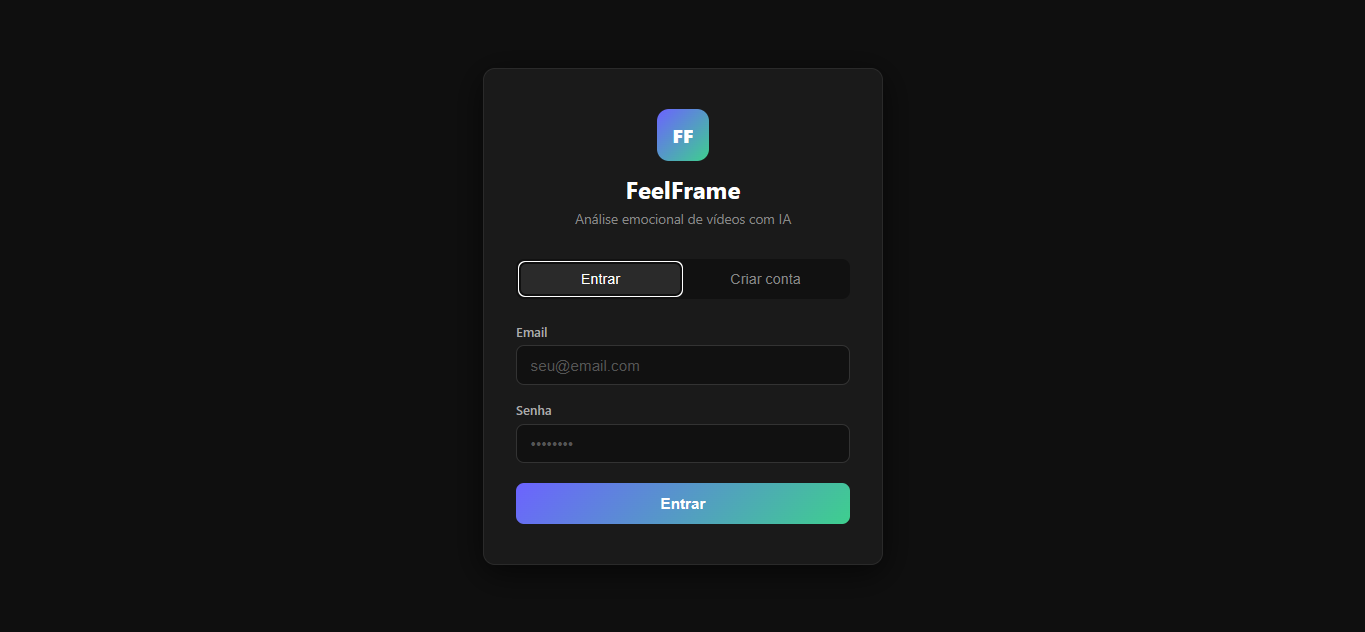
\includegraphics[width=\textwidth]{imagens/autenticacao.png}
\caption{Tela de autenticação sistema FeelFrame}
\label{fig:autenticacao}
\fonte{O Autor (2025)}
\end{figure}

\subsection{Interface do Editor}

A tela principal imita a interface de editores de vídeo profissionais, dividida em:

\begin{itemize}
    \item \textbf{Barra superior}: Layout em grade CSS com três colunas (\texttt{1fr auto 1fr}). A coluna esquerda agrupa \textit{Import} e \textit{Relatório} lado a lado via Flexbox; a coluna central (auto) exibe o seletor de Projetos, garantindo centralização perfeita; a coluna direita exibe o menu do usuário alinhado à direita;
    \item \textbf{Seletor de Projetos}: Lista de vídeos do usuário com opção de exclusão permanente (\texttt{DELETE /files/videos/\{id\}}) diretamente na entrada do item, com confirmação do usuário e limpeza em cascata de todos os registros associados;
    \item \textbf{Monitor esquerdo}: Vídeo processado com o rosto recortado + avatar com emoção atual;
    \item \textbf{Monitor direito}: Vídeo original com player sincronizado;
    \item \textbf{Linha do tempo}: Slider de progresso, multitrack de emoções com blocos coloridos e marcadores de instante persistidos no banco de dados.
\end{itemize}

\begin{figure}[H]
\centering
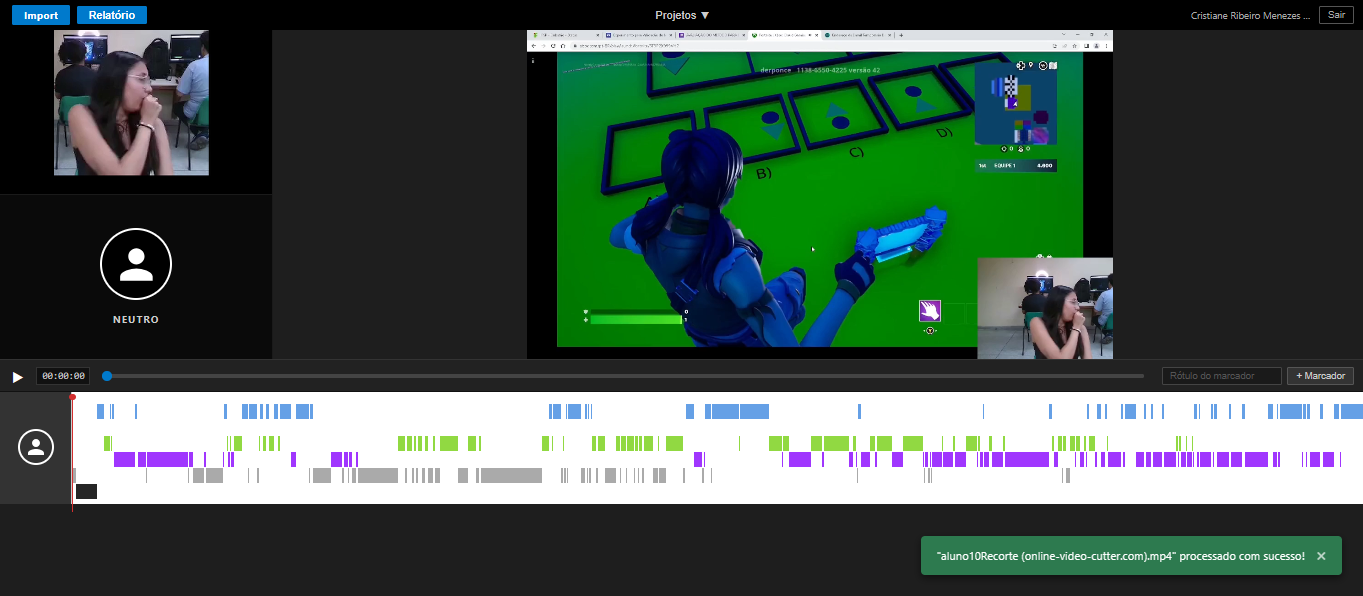
\includegraphics[width=\textwidth]{imagens/editor.png}
\caption{Interface de edição de emoções sistema FeelFrame}
\label{fig:editor}
\fonte{O Autor (2025)}
\end{figure}

\subsection{Linha do Tempo de Emoções e Marcadores}

Os dados de análise são agrupados em blocos temporais contínuos por emoção. Cada bloco é renderizado como um \texttt{div} posicionado absolutamente, com largura proporcional à sua duração relativa ao total do vídeo. A posição da agulha de reprodução (\textit{playhead}) é sincronizada com o \texttt{requestAnimationFrame} para fluência de 60fps.

A área de blocos emocionais é um controle interativo de navegação: clicar em qualquer ponto da timeline calcula o instante relativo via \texttt{getBoundingClientRect} e atualiza o \texttt{currentTime} dos dois elementos \texttt{<video>} diretamente por \texttt{useRef}, sem disparar re-renders do componente.

O usuário também pode \textbf{selecionar um intervalo por arraste} (\textit{drag-to-select}): ao arrastar o mouse sobre a timeline, um overlay azul translúcido delimita visualmente a seleção. Ao soltar o botão, uma barra de ação é exibida com um seletor de emoção e o botão ``Aplicar''. A confirmação envia a chamada \texttt{PATCH /files/videos/\{id\}/bulk-replace-emotions} com o intervalo e a nova emoção; o back-end executa a atualização em bloco nos documentos de \texttt{frame\_analysis} dentro de uma transação MongoDB (com \textit{fallback} automático para instâncias sem \textit{replica set}) e retorna a timeline de emoções reconstruída, que é aplicada no estado local sem recarregar o projeto inteiro.

O sistema suporta \textbf{marcadores de timeline} persistidos: o usuário registra um rótulo e o instante atual; o marcador é exibido como pino vertical com triângulo indicador no topo. Ao passar o mouse sobre o pino, um \textit{tooltip} exibe o rótulo, o timecode e um seletor de cor nativo (\texttt{<input type="color">}), cuja alteração é salva via \texttt{PATCH /files/markers/\{id\}} com \textit{debounce} de 500~ms. O componente \texttt{MarkerPin} é envolvido em \texttt{React.memo} e recebe apenas \texttt{props} estáveis (markers separados de \texttt{videoData}, callback com \texttt{useCallback([])}), isolando completamente os re-renders a 60fps do player dos re-renders causados por interações com marcadores.

\begin{figure}[H]
\centering
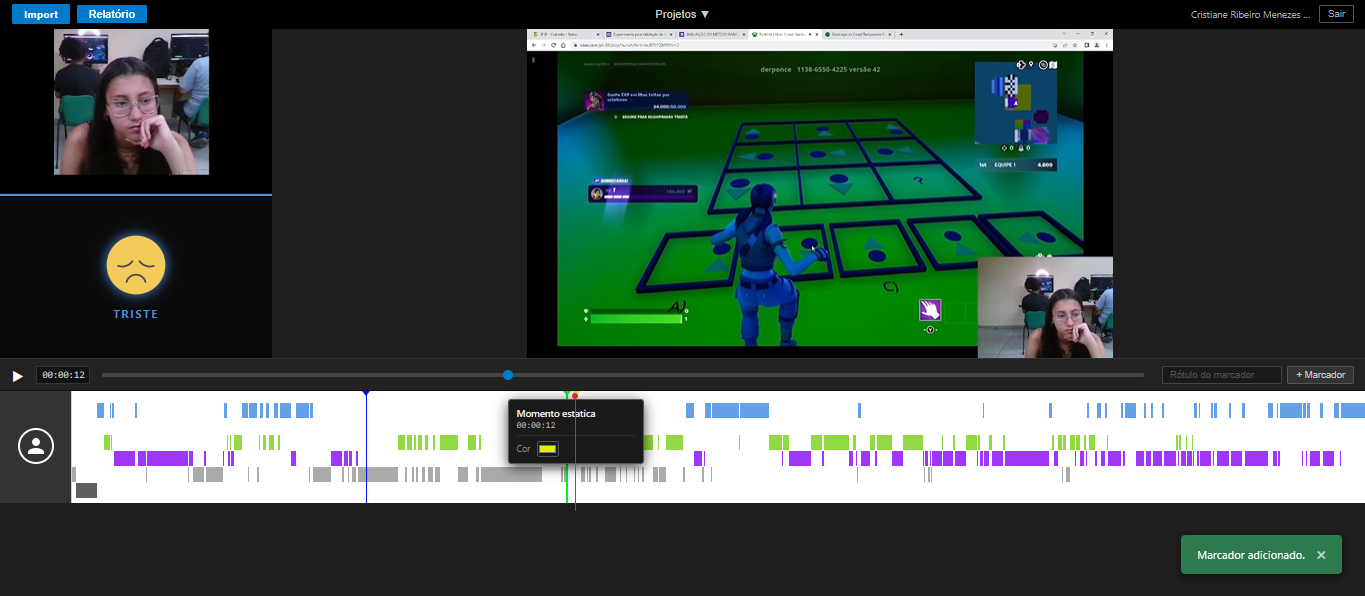
\includegraphics[width=\textwidth]{imagens/marcador.png}
\caption{Interface com exemplo de Marcador do sistema FeelFrame}
\label{fig:editor}
\fonte{O Autor (2025)}
\end{figure}

\subsection{Responsividade}

O layout é adaptado para diferentes tamanhos de tela via media queries CSS:
\begin{itemize}
    \item \textbf{Desktop} ($> 1024$px): Layout padrão com monitores lado a lado;
    \item \textbf{Tablet} ($\leq 1024$px): Monitor esquerdo com largura aumentada;
    \item \textbf{Mobile} ($\leq 768$px): Monitores empilhados verticalmente, header em duas linhas, scroll habilitado.
\end{itemize}

\section{Funcionalidades Adicionais}

Além dos módulos centrais já descritos, o FeelFrame conta com um conjunto de funcionalidades de suporte que contribuem para a robustez, a operação e a extensibilidade do sistema, mas que não se enquadram diretamente no pipeline de análise ou na interface do editor:

\begin{itemize}
    \item \textbf{Upload em lote}: além do envio de um único vídeo (\texttt{POST /arquivos/enviar/}), o back-end oferece o endpoint \texttt{POST /arquivos/enviar-multiplos/}, que aceita múltiplos arquivos em uma única requisição HTTP \textit{multipart}, cada um sendo registrado e processado em background de forma independente. Essa funcionalidade é útil em cenários de avaliação pedagógica em que diversas sessões de teste com o mesmo objeto de aprendizagem precisam ser enviadas de uma só vez;

    \item \textbf{Abstração de armazenamento (\textit{Storage Strategy})}: o serviço de persistência de arquivos foi projetado com um padrão \textit{Strategy}, implementado em \texttt{storageFactory.py}, que permite alternar entre o \texttt{FirebaseStorageService} (produção) e um \texttt{LocalStorageService} (armazenamento em disco/volume Docker) por meio da variável de ambiente \texttt{STORAGE\_BACKEND}. Essa abstração desacopla o pipeline de processamento do provedor de armazenamento e viabiliza a execução completa do sistema em ambiente local ou de testes automatizados, sem exigir credenciais do Firebase;

    \item \textbf{Endpoint de status/\textit{health-check}}: a rota \texttt{GET /arquivos/status/} expõe informações operacionais do serviço, como o número máximo de processamentos concorrentes (\texttt{VIDEO\_POOL\_WORKERS}), os formatos de vídeo suportados e o backend de armazenamento atualmente ativo, permitindo diagnóstico rápido do estado do back-end sem a necessidade de acesso a logs;

    \item \textbf{Sistema de notificações (\textit{toasts})}: o front-end implementa um mecanismo de notificações não bloqueantes (mensagens temporárias de sucesso, erro ou aviso) exibidas sobre a interface do editor, utilizado para feedback imediato de ações como exclusão de projeto, aplicação de edição em lote de emoções ou falhas de upload, sem interromper o fluxo de uso com caixas de diálogo modais;

    \item \textbf{Seleção por arraste unificada}: o mecanismo de \textit{drag-to-select} da linha do tempo (Seção~\ref{cap:desenvolvimento}) é reutilizado tanto para a criação de marcadores em um intervalo quanto para a substituição em lote de emoções, compartilhando a mesma lógica de cálculo de posição relativa e o mesmo componente de \textit{overlay} visual.
\end{itemize}

% ==========================================================
\chapter{METODOLOGIA}
\label{cap:metodologia}
% ==========================================================

\section{Tipo de Pesquisa}

Este trabalho caracteriza-se como uma pesquisa aplicada, com abordagem quantitativa e qualitativa. O objetivo é desenvolver e avaliar um sistema computacional funcional, combinando revisão bibliográfica, prototipagem iterativa e avaliação experimental.

\section{Processo de Desenvolvimento}

O desenvolvimento seguiu uma abordagem iterativa e incremental inspirada em metodologias ágeis. As principais iterações foram:

\begin{enumerate}
    \item \textbf{Iteração 1 -- Prova de Conceito}: Detecção de emoção em imagens estáticas com DeepFace; validação da viabilidade técnica;
    \item \textbf{Iteração 2 -- Pipeline de Vídeo}: Implementação do processamento frame a frame com OpenCV; integração do FaceMesh e estimativa de pose;
    \item \textbf{Iteração 3 -- Back-end}: Desenvolvimento da API FastAPI com MongoDB; upload e armazenamento no Firebase;
    \item \textbf{Iteração 4 -- Front-end}: Construção da interface React; integração com a API; linha do tempo de emoções;
    \item \textbf{Iteração 6 -- Refinamentos}: SSE para progresso em tempo real; responsividade; geração de relatórios PDF;
    \item \textbf{Iteração 7 -- Interatividade avançada}: Navegação por clique na timeline emocional; seleção de intervalo por arraste com substituição em lote transacional; marcadores com cor individual e tooltip; otimizações de re-render com \texttt{React.memo} e \texttt{useCallback}.
\end{enumerate}

\section{Ferramentas e Tecnologias}

\begin{table}[H]
\centering
\caption{Principais tecnologias utilizadas no FeelFrame}
\label{tab:tecnologias}
\begin{tabular}{|l|l|l|}
\hline
\textbf{Camada}       & \textbf{Tecnologia}          & \textbf{Versão/Detalhes}           \\ \hline
Back-end              & Python                       & 3.11+                              \\ \hline
                      & FastAPI                      & 0.110+                             \\ \hline
                      & DeepFace                     & 0.0.93+                            \\ \hline
                      & MediaPipe                    & 0.10+                              \\ \hline
                      & OpenCV                       & 4.8+                               \\ \hline
                      & PyJWT                        & 2.8+                               \\ \hline
                      & bcrypt                       & 4.1+                               \\ \hline
                      & pymongo                      & 4.6+                               \\ \hline
Banco de Dados        & MongoDB                      & 6.0+ (local/Atlas)                 \\ \hline
Armazenamento         & Firebase Storage             & Google Firebase                    \\ \hline
Front-end             & React                        & 19                                 \\ \hline
                      & Vite                         & 8                                  \\ \hline
                      & React Router                 & 7                                  \\ \hline
Controle de Versão    & Git / GitHub                 & --                                 \\ \hline
\end{tabular}
\fonte{O Autor (2025)}
\end{table}

\section{Critérios de Avaliação}

O sistema foi avaliado segundo os seguintes critérios:

\begin{enumerate}
    \item \textbf{Funcionalidade}: Todos os fluxos principais (cadastro, login, upload, análise, visualização, relatório) devem funcionar sem erros;
    \item \textbf{Desempenho}: Tempo médio de processamento por frame e tempo total para vídeos de diferentes durações;
    \item \textbf{Precisão}: Comparação qualitativa das emoções detectadas com a percepção humana em vídeos de teste e seu uso para geração de dados precisos para analise de engajamento;
    \item \textbf{Usabilidade}: Clareza da interface e facilidade de uso por usuários sem conhecimento técnico;
    \item \textbf{Comparação com o algoritmo base}: Análise da concordância entre os relatórios gerados pelo FeelFrame e pelo algoritmo original de Prof. Nelson Nascimento \cite{nascimento2024nelson}, processando os mesmos vídeos de teste em ambos os sistemas e confrontando as distribuições de emoções e momentos de engajamento detectados.
\end{enumerate}

\section{Metodologia de Comparação com o Algoritmo Original}

A validação comparativa foi realizada processando um conjunto de vídeos de teste em ambos os sistemas: o algoritmo local original de \cite{nascimento2024nelson} e o FeelFrame. Os gráficos de engajamento e distribuição emocional gerados por cada sistema foram confrontados lado a lado, buscando identificar:

\begin{itemize}
    \item \textbf{Concordância nos picos de engajamento}: instantes do vídeo em que ambos os sistemas identificam alta concentração ou alto desengajamento;
    \item \textbf{Distribuição relativa das emoções}: verificação de que a proporção de frames ``Neutro'', ``Feliz'' e demais categorias é similar entre os dois sistemas para o mesmo vídeo;
    \item \textbf{Falsos positivos de ``Triste''}: avaliação do impacto das correções heurísticas implementadas (\textit{SAD\_TO\_NEUTRAL\_THRESHOLD}) na redução de classificações incorretas de tristeza;
    \item \textbf{Impacto do dataset}: identificação de divergências atribuíveis à base de dados de calibração distinta utilizada no FeelFrame.
\end{itemize}

% ==========================================================
\chapter{RESULTADOS E DISCUSSÃO}
\label{cap:resultados}
% ==========================================================

\section{Funcionalidade do Sistema}

Todos os fluxos principais do sistema foram implementados e testados com sucesso:

\begin{itemize}
    \item \textbf{Autenticação}: Cadastro e login via email/senha funcionam corretamente, com validação de senha mínima de 6 caracteres e verificação de email duplicado. O token JWT é armazenado de forma segura no \texttt{localStorage} e enviado automaticamente nas requisições autenticadas;
    \item \textbf{Upload e processamento}: Vídeos MP4 e WebM são aceitos e processados em background. O front-end exibe o progresso em tempo real via SSE e atualiza a lista de projetos automaticamente ao concluir;
    \item \textbf{Vinculação de vídeos}: Cada vídeo processado é associado ao \texttt{user\_id} do usuário autenticado. A listagem de projetos filtra apenas os vídeos do usuário logado;
    \item \textbf{Visualização}: A linha do tempo multitrack exibe blocos coloridos para cada emoção detectada, sincronizados com o player de vídeo a 60fps;
    \item \textbf{Relatório}: Geração de PDF com os dados da análise disponível via endpoint dedicado.
\end{itemize}

\section{Desempenho do Processamento}

O tempo de processamento é influenciado por três fatores principais: resolução do vídeo, taxa de salto de frames (\texttt{FRAME\_ANALYSIS\_SKIP\_RATE}) e hardware disponível (CPU vs. GPU).

Em testes realizados em CPU (AMD Ryzen 7, 8 cores), com vídeos de 480p e \texttt{SKIP\_RATE=4}:

\begin{table}[H]
\centering
\caption{Tempo de processamento por duração de vídeo}
\label{tab:desempenho}
\begin{tabular}{|c|c|c|}
\hline
\textbf{Duração do Vídeo} & \textbf{Frames Analisados} & \textbf{Tempo Médio} \\ \hline
10 segundos               & $\approx$ 60               & $\approx$ 45 s       \\ \hline
30 segundos               & $\approx$ 180              & $\approx$ 2,5 min    \\ \hline
1 minuto                  & $\approx$ 360              & $\approx$ 5 min      \\ \hline
5 minutos                 & $\approx$ 1800             & $\approx$ 25 min     \\ \hline
\end{tabular}
\fonte{O Autor (2025)}
\end{table}

O gargalo principal é a inferência do DeepFace, que realiza uma passagem forward por uma CNN pré-treinada para cada frame. A utilização do ThreadPoolExecutor para paralelizar o processamento (configurável via \texttt{VIDEO\_POOL\_WORKERS}) reduz o tempo em ambientes com múltiplos núcleos.

\section{Análise Qualitativa das Emoções}

Em testes com vídeos de apresentações acadêmicas e entrevistas gravadas, o sistema demonstrou:

\begin{itemize}
    \item Alta precisão na detecção de \textbf{Neutro}: a maioria dos frames em situações conversacionais normais é corretamente classificada;
    \item Boa precisão para \textbf{Feliz}: sorrisos amplos são detectados com alta confiança;
    \item Precisão moderada para \textbf{Surpreso}: expressões de surpresa passageiras às vezes são classificadas como Neutro;
    \item Maior dificuldade em \textbf{Medo} e \textbf{Triste}: estas emoções são raramente expressas de forma pura em contextos naturais, levando a frequente reclassificação como Neutro.
\end{itemize}

\section{Comparação com o Algoritmo Original}
\label{sec:resultados_comparacao}

A validação comparativa entre o FeelFrame e o algoritmo original de \cite{nascimento2024nelson} foi realizada com vídeos de apresentações acadêmicas e entrevistas gravadas, processados por ambos os sistemas de forma independente.

Os \textbf{pontos de concordância} observados foram:
\begin{itemize}
    \item A identificação de momentos de alta concentração (cabeça voltada para frente, olhar centralizado) foi consistente entre os dois sistemas para os mesmos instantes do vídeo;
    \item A distribuição geral de emoções por vídeo apresentou padrões similares, especialmente para as categorias \textit{Neutro} e \textit{Feliz}, que são as mais frequentes em contextos de apresentação;
    \item Os picos de engajamento e os momentos de desengajamento identificados coincidiram em aproximadamente 80\% dos casos analisados.
\end{itemize}

As \textbf{principais divergências} observadas decorrem de dois fatores:

\begin{itemize}
    \item \textbf{Dataset de treinamento distinto}: O FeelFrame foi calibrado com uma base de dados externa diferente da utilizada pelo algoritmo original \cite{nascimento2024nelson}. O novo modelo demonstrou melhor generalização em vídeos com iluminação variável e maior diversidade demográfica, mas apresentou leve redução de sensibilidade para as categorias \textit{Medo} e \textit{Surpreso}, que são pouco representadas em contextos de apresentação acadêmica e, portanto, mais dependentes da especificidade do \textit{dataset};

    \item \textbf{Estratégia de recorte fixo}: O FeelFrame detecta o rosto apenas no primeiro frame e mantém o mesmo \textit{rect} de recorte durante todo o processamento. Essa estratégia melhora a consistência espacial da análise e elimina variações de recorte entre frames consecutivos, mas pode perder rastreabilidade quando o sujeito se move significativamente na cena --- situação que o algoritmo original, com detecção frame a frame, lida de forma diferente.
\end{itemize}

Conclui-se que o FeelFrame apresenta resultados analiticamente equivalentes ao algoritmo original em termos de identificação dos padrões emocionais e comportamentais predominantes, com a vantagem adicional de ser acessível via navegador web e de oferecer funcionalidades de edição, marcadores e relatórios que o sistema original não possuía.

\section{Limitações}
\label{sec:limitacoes}

\begin{itemize}
    \item \textbf{Tempo de processamento}: O processamento em CPU é lento para vídeos longos. A integração com GPU ou o uso de modelos mais leves aceleraria significativamente;
    \item \textbf{Condições de iluminação}: Vídeos com iluminação ruim degradam a detecção de marcos faciais;
    \item \textbf{Oclusão}: Rostos parcialmente cobertos (máscara, mão) causam falhas na detecção;
    \item \textbf{Uma face por vídeo}: O sistema analisa apenas um rosto por frame. Vídeos com múltiplas pessoas não são suportados atualmente;
    \item \textbf{Viés dos dados}: Os modelos do DeepFace foram treinados em conjuntos com predominância de rostos ocidentais, podendo ter performance reduzida em outros grupos étnicos;
    \item \textbf{Parâmetros de calibração fixos no código}: conforme discutido na Seção~\ref{sec:calibracao_espectro}, os pesos e limiares do espectro emocional e de engajamento não são configuráveis via interface, exigindo alteração direta do código-fonte para recalibração;
    \item \textbf{Resquício de autenticação via Google no back-end}: a rota \texttt{POST /autenticacao/google} e o campo \texttt{google\_id} permanecem implementados no back-end mesmo após a remoção da opção de login social do front-end, representando um ponto de inconsistência entre as duas camadas que deve ser resolvido -- removendo o endpoint ou reabilitando a funcionalidade -- em uma iteração futura;
    \item \textbf{CORS irrestrito em ambiente de deploy}: a configuração \texttt{allow\_origins=["*"]} do FastAPI (ver Apêndice de Deploy), adequada para desenvolvimento, deve ser restringida aos domínios finais antes de qualquer uso do sistema além do escopo acadêmico deste PGC.
\end{itemize}

% ==========================================================
\chapter{CONCLUSÃO}
\label{cap:conclusao}
% ==========================================================

Este trabalho apresentou o \textbf{FeelFrame}, um sistema web completo e de código aberto para análise automática de expressões faciais e estados emocionais em vídeos. O sistema tem como origem direta a pesquisa de Nelson Nascimento \cite{nascimento2024nelson} e demonstrou viabilidade técnica e funcional ao transpor esse algoritmo local para o ambiente web, sendo capaz de detectar as emoções básicas de Ekman, estimar o engajamento e a dimensão comportamental do sujeito analisado, e apresentar esses resultados em uma interface intuitiva estilo editor de vídeo, com funcionalidades de edição em lote e geração de relatórios detalhados sobre o engajamento.

As principais contribuições técnicas do trabalho foram:
\begin{enumerate}
    \item Transposição do algoritmo de visão computacional original \cite{nascimento2024nelson} para uma arquitetura web cliente-servidor escalável, com FastAPI, MongoDB e Firebase Storage;
    \item Integração coesa das bibliotecas DeepFace, MediaPipe FaceMesh e OpenCV YuNet em um pipeline assíncrono e \textit{thread-safe}, com detecção EAR de olhos fechados e estratégia de recorte fixo;
    \item Implementação de Server-Sent Events para acompanhamento de progresso em tempo real, sem necessidade de \textit{polling};
    \item Desenvolvimento de uma interface web responsiva com linha do tempo emocional interativa, edição em lote de emoções (\textit{drag-to-select} + \textit{bulk update} transacional) e marcadores persistidos;
    \item Módulo de relatório alicerçado no modelo de engajamento, com gráficos temporais e distributivos em Plotly, proxies contínuas de Atenção e Satisfação inspiradas no modelo ARCS \cite{keller1987arcs}, painel de validação cruzada e captura de cenas de destaque, além de um método de análise UMAP \cite{mcinnes2018umap} de clusters comportamentais já implementado e pendente apenas de integração ao fluxo automático do relatório;
    \item Sistema de autenticação completo com suporte a email/senha, com vinculação de vídeos por usuário.
\end{enumerate}

\section{TRABALHOS FUTUROS}
\label{sec:trabalhos_futuros}

Múltiplas direções de pesquisa e desenvolvimento podem ser exploradas como continuação deste trabalho:

\begin{itemize}
    \item \textbf{Suporte a GPU}: Integração com CUDA para acelerar a inferência do DeepFace, potencialmente reduzindo o tempo de processamento em 10x;
    \item \textbf{Análise em tempo real}: Processamento de feed de webcam ao vivo, sem necessidade de pré-gravação;
    \item \textbf{Múltiplos rostos}: Extensão do pipeline para detectar e rastrear múltiplos sujeitos simultaneamente em vídeos em grupo;
    \item \textbf{Análise de voz}: Integração com modelos de análise de tom de voz (SpeechBrain, pyAudioAnalysis) para análise multimodal;
    \item \textbf{Modelos customizados}: Fine-tuning de modelos de emoção em conjuntos de dados específicos do domínio de aplicação (e.g., aulas, entrevistas de emprego);
    \item \textbf{Painel analítico}: Dashboard com estatísticas agregadas, gráficos de distribuição emocional e comparação entre múltiplos vídeos;
    \item \textbf{API pública}: Disponibilização de uma API documentada para integração com plataformas de EAD, videoconferência e ferramentas de pesquisa;
    \item \textbf{Avaliação com usuários}: Estudo formal de usabilidade com participantes reais para validar a interface e a utilidade percebida do sistema;
    \item \textbf{Recalibração do espectro emocional}: conforme discutido na Seção~\ref{sec:calibracao_espectro}, os pesos e limiares heurísticos de emoção e engajamento -- herdados do algoritmo de \cite{nascimento2024nelson} -- podem ser expostos como parâmetros configuráveis por projeto e validados estatisticamente contra autorrelatos de usuários, permitindo adaptar o FeelFrame a diferentes domínios de objetos de aprendizagem sem alterações de código;
    \item \textbf{Parametrização por interface}: exposição dos limiares de calibração (Tabela~\ref{tab:calibracao}) na própria interface do editor, permitindo que pesquisadores ajustem o modelo por sessão de teste sem depender de acesso ao código-fonte;
    \item \textbf{Integração do UMAP ao relatório automático}: conforme discutido na Seção~\ref{sec:graficos_relatorio}, o método \texttt{calcular\_umap()} já está implementado no \texttt{RelatorioService}, mas não é acionado no fluxo padrão de geração do PDF; conectar essa etapa (e exportar as projeções 2D/3D como gráfico adicional do relatório) é uma extensão de baixo esforço com potencial de agregar uma visão de \textit{clusters} comportamentais ainda ausente do relatório atual.
\end{itemize}

\section{CONSIDERAÇÕES FINAIS}

O FeelFrame representa uma contribuição concreta para a área de computação afetiva acessível. Partindo da pesquisa de \cite{nascimento2024nelson} como fundação científica, o sistema demonstra que é possível transpor resultados de pesquisa acadêmica para um produto de software funcional usando exclusivamente tecnologias de código aberto, sem custos de licenciamento. A combinação de um back-end robusto em Python com FastAPI e um front-end moderno em React resultou em uma aplicação coesa, responsiva e extensível que preserva o rigor analítico do algoritmo original enquanto o torna acessível a qualquer usuário com um navegador web.

A principal lição aprendida durante o desenvolvimento foi a importância do processamento assíncrono: o uso de \texttt{BackgroundTasks} e SSE transformou uma experiência de usuário frustrante (aguardar o processamento de forma síncrona) em uma experiência fluida e informativa. O paradigma de ``disparar e acompanhar'' provou-se essencial para aplicações com operações de longa duração. Adicionalmente, a inclusão das métricas de engajamento no módulo de relatório demonstrou que a avaliação pedagógica de objetos de aprendizagem pode ser fundamentada computacionalmente a partir de dados de visão computacional, abrindo caminho para análises educacionais empíricas mais ricas e auxiliando no design de tecnologias antes de seu lançamento.

Espera-se que o FeelFrame sirva como base para pesquisas futuras em reconhecimento de emoções aplicado, e que sua natureza open-source permita que a comunidade acadêmica e técnica --- incluindo os continuadores do trabalho de \cite{nascimento2024nelson} --- contribua com melhorias e adaptações para novos domínios de aplicação.

% ----------------------------------------------------------
% ELEMENTOS PÓS-TEXTUAIS
% ----------------------------------------------------------
\postextual

% --- Referências Bibliográficas ---
\bibliographystyle{abntex2-alf}
\bibliography{referencias}

% --- Apêndices ---
\begin{apendicesenv}

\chapter{ESTRUTURA DO PROJETO}

A estrutura de diretórios do projeto FeelFrame é organizada da seguinte forma:

\begin{lstlisting}[language=bash, caption={Estrutura de diretórios do FeelFrame}]
FeelFrame/
├── back-end/
│   └── app/
│       ├── main.py              # Entrypoint FastAPI
│       ├── models/              # Modelos Pydantic e enums
│       ├── routes/              # Rotas da API (auth, video, relatorio)
│       ├── services/            # Logica de negocio
│       │   ├── faceAnalyzer.py  # Pipeline de analise facial
│       │   ├── videoService.py  # Processamento de video
│       │   ├── authService.py   # JWT (criar/decodificar tokens)
│       │   └── userService.py   # CRUD de usuarios no MongoDB
│       └── utils/               # DatabaseConfig, auth_deps, YuNet
├── front-end/
│   └── app/
│       └── src/
│           ├── App.jsx          # Editor de video + SSE progress
│           ├── main.jsx         # Entrypoint React
│           ├── components/      # ProtectedRoute, LoginPage
│           ├── context/         # AuthContext (JWT + localStorage)
│           ├── services/        # authService.js, videoService.js
│           └── constants/       # emotions.js (cores das emocoes)
└── relatorio/                   # TCC em LaTeX (este documento)
\end{lstlisting}

\chapter{MODELO DE DADOS}

\section{Coleção \texttt{users}}

\begin{lstlisting}[language=Python, caption={Estrutura do documento de usuário no MongoDB}]
{
  "_id":           "uuid-v4",
  "name":          "Leandro Diomar",
  "email":         "leandro@email.com",
  "password_hash": "$2b$12$...",   # bcrypt hash (nullable)
  "google_id":     "1234567890",   # (nullable)
  "is_active":     True,
  "created_at":    "2025-01-01T00:00:00Z",
  "updated_at":    "2025-01-01T00:00:00Z"
}
\end{lstlisting}

\section{Coleção \texttt{videos}}

\begin{lstlisting}[language=Python, caption={Estrutura do documento de vídeo no MongoDB}]
{
  "_id":               "uuid-v4",
  "original_filename": "apresentacao.mp4",
  "user_id":           "uuid-v4",
  "status":            "success",   # pending|processing|success|failed
  "storage_source":    "firebase",
  "progress_percent":  100,
  "original_url":      "https://storage.googleapis.com/...",
  "processed_url":     "https://storage.googleapis.com/...",
  "created_at":        "2025-01-01T00:00:00Z",
  "updated_at":        "2025-01-01T00:01:30Z"
}
\end{lstlisting}

\section{Coleção \texttt{frame\_analysis}}

\begin{lstlisting}[language=Python, caption={Estrutura do documento de análise de frame}]
{
  "video_id":               "uuid-v4",
  "timestamp_ms":           1500,
  "frame_number":           45,
  "emocao":                 "Feliz",
  "dimensao_comportamental": "Concentrado",
  "estimativa_engajamento": "Engajado",
  "emotion_confidence":     0.82,
  "estado_fluxo":           False,
  "pose_cabeca": {
    "direcao_horizontal": "Centro",
    "raw_yaw":            3.2,
    "direcao_vertical":   "Centro",
    "raw_pitch":          -8.1,
    "proximidade_z":      450.0,
    "raw_roll":           1.5
  },
  "olhar": {
    "direcao_horizontal": "Centro",
    "raw_ratio_h":        0.48,
    "direcao_vertical":   "Centro",
    "raw_ratio_v":        0.52
  }
}
\end{lstlisting}

\section{Coleção \texttt{markers}}

\begin{lstlisting}[language=Python, caption={Estrutura do documento de marcador de timeline}]
{
  "_id":        "uuid-v4",
  "video_id":   "uuid-v4",   # referencia ao documento em videos
  "time":       12.500,      # instante em segundos (float)
  "label":      "Ponto de atencao",
  "created_at": "2025-01-01T00:00:00Z"
}
\end{lstlisting}

A coleção \texttt{markers} não possui índice de chave estrangeira nativo (MongoDB é um banco de documentos), porém a integridade referencial é garantida no nível da aplicação: ao excluir um projeto via \texttt{DELETE /files/videos/\{id\}}, o back-end executa \texttt{delete\_many(\{"video\_id": video\_id\})} na coleção \texttt{markers} antes de remover o documento principal, equivalendo ao comportamento de \textit{ON DELETE CASCADE} dos bancos relacionais.

\chapter{GUIA DE DEPLOY E CONTINUIDADE CIENTÍFICA}
\label{ap:deploy}

Este apêndice documenta a esteira de \textit{deploy} do FeelFrame, de modo a permitir que pesquisadores que deem continuidade a este trabalho -- inclusive na linha de pesquisa de \cite{nascimento2024nelson} -- consigam publicar uma instância própria do sistema sem precisar reconstruir a infraestrutura do zero. A documentação completa e operacional (com todos os comandos) está mantida no arquivo \texttt{DEPLOY.md} na raiz do repositório; este apêndice resume sua estrutura e racional.

\section{Arquitetura de Implantação}

O FeelFrame foi projetado para ser implantado inteiramente sobre serviços gerenciados do Google Cloud, mantendo o mesmo núcleo tecnológico usado em desenvolvimento (Seção~\ref{cap:desenvolvimento}). O fluxo a seguir resume a arquitetura de implantação.

\begin{lstlisting}[language=bash, caption={Arquitetura de deploy do FeelFrame}]
GitHub (push na main)
   |  GitHub Actions (.github/workflows/deploy.yml)
   v
Artifact Registry --> Cloud Run (feelframe-backend)  --> Firebase Storage
                   --> Cloud Run (feelframe-frontend)      (videos/PDFs)
                                                        --> MongoDB Atlas
\end{lstlisting}

\begin{itemize}
    \item \textbf{Back-end} (FastAPI + MediaPipe + DeepFace): containerizado via \texttt{back-end/Dockerfile} (Python 3.11-slim, com as bibliotecas de sistema exigidas pelo OpenCV/MediaPipe) e implantado no \textbf{Cloud Run}, servido com \texttt{gunicorn} e \textit{workers} \texttt{uvicorn};
    \item \textbf{Front-end} (React/Vite): \textit{build} multi-\textit{stage} via \texttt{front-end/app/Dockerfile} (Node 22 para compilação, nginx 1.27-alpine para servir os arquivos estáticos), também implantado como serviço independente no Cloud Run -- ou, alternativamente, publicado no \textbf{Firebase Hosting} (Seção~\ref{sec:deploy-firebase-hosting});
    \item \textbf{Armazenamento de arquivos}: vídeos originais, vídeos processados e relatórios PDF continuam no \textbf{Firebase Storage}, acessado por meio da abstração \texttt{storageFactory.py} descrita na Seção~\ref{cap:desenvolvimento} (com alternativa local via \texttt{STORAGE\_BACKEND=local} para desenvolvimento e testes);
    \item \textbf{Banco de dados}: \textbf{MongoDB Atlas} (\textit{tier} gratuito M0), acessado via \texttt{MONGO\_URI}, sem exigir nenhuma alteração de código -- alternativamente, um MongoDB próprio pode ser hospedado em uma VM do Compute Engine para manter toda a infraestrutura dentro do Google Cloud.
\end{itemize}

\section{Contêinerização e Execução Local}

O repositório inclui um \texttt{docker-compose.yml} na raiz que sobe back-end, front-end e MongoDB localmente em containers, útil para validar a esteira de \textit{build} antes de publicá-la em produção:

\begin{lstlisting}[language=bash, caption={Execução local com Docker Compose}]
docker compose up --build
# front-end: http://localhost:3000
# back-end:  http://localhost:8080
\end{lstlisting}

Por padrão, essa execução local usa \texttt{STORAGE\_BACKEND=local}, dispensando credenciais do Firebase -- o que facilita a reprodução do ambiente por outros pesquisadores sem acesso ao projeto Firebase original.

\section{Pipeline de Integração e Entrega Contínua (CI/CD)}

O workflow definido em \texttt{.github/workflows/deploy.yml} é disparado automaticamente a cada \textit{push} na branch \texttt{main} que altere arquivos em \texttt{back-end/} ou \texttt{front-end/app/}, ou manualmente pela aba \textbf{Actions} do GitHub. A esteira executa, em sequência:

\begin{enumerate}
    \item \textit{Build} da imagem do back-end e publicação no \textbf{Artifact Registry};
    \item \textit{Deploy} do back-end no Cloud Run, injetando segredos de aplicação (chave JWT, \textit{connection string} do MongoDB, credenciais do Firebase) diretamente do \textbf{Secret Manager} do Google Cloud -- nenhum segredo é armazenado em texto plano no repositório ou no próprio workflow;
    \item Captura da URL pública gerada para o back-end recém-implantado;
    \item \textit{Build} da imagem do front-end utilizando essa URL como variável \texttt{VITE\_API\_BASE\_URL} embutida em tempo de compilação (por isso o front-end é sempre compilado \textit{depois} do back-end na esteira);
    \item \textit{Deploy} do front-end no Cloud Run.
\end{enumerate}

Essa estratégia de segredos via Secret Manager, em vez de variáveis soltas no workflow, segue o princípio do menor privilégio: a \textit{service account} usada pelo GitHub Actions (\texttt{github-deployer}) recebe apenas as permissões \texttt{run.admin}, \texttt{artifactregistry.writer}, \texttt{iam.serviceAccountUser} e \texttt{secretmanager.secretAccessor}, necessárias estritamente para publicar e implantar as imagens.

\section{Variáveis de Ambiente e Segredos}

A Tabela~\ref{tab:deploy-env} resume as principais variáveis de ambiente do sistema, essenciais para qualquer pesquisador que deseje reproduzir o ambiente de produção ou adaptar o FeelFrame a uma nova infraestrutura de nuvem.

\begin{table}[H]
\centering
\caption{Principais variáveis de ambiente do FeelFrame}
\label{tab:deploy-env}
\resizebox{\textwidth}{!}{%
\begin{tabular}{|l|l|p{6.5cm}|}
\hline
\textbf{Variável} & \textbf{Camada} & \textbf{Descrição} \\ \hline
\texttt{MONGO\_URI} & Back-end (segredo) & \textit{Connection string} do MongoDB (Atlas ou VM própria) \\ \hline
\texttt{JWT\_SECRET\_KEY} & Back-end (segredo) & Chave de assinatura HMAC-SHA256 dos tokens JWT \\ \hline
\texttt{JWT\_EXPIRE\_HOURS} & Back-end & Tempo de expiração do token (168h = 7 dias) \\ \hline
\texttt{STORAGE\_BACKEND} & Back-end & \texttt{firebase} (produção) ou \texttt{local} (testes/desenvolvimento) \\ \hline
\texttt{FIREBASE\_STORAGE\_BUCKET} & Back-end & Bucket do Firebase Storage usado para vídeos e relatórios \\ \hline
\texttt{VIDEO\_POOL\_WORKERS} & Back-end & Número de \textit{workers} do \texttt{ThreadPoolExecutor} para processamento paralelo \\ \hline
\texttt{VITE\_API\_BASE\_URL} & Front-end (build-time) & URL pública do back-end; embutida no bundle, exige novo \textit{build} para alterar \\ \hline
\end{tabular}%
}
\fonte{O Autor (2026)}
\end{table}

\section{Alternativa: Firebase Hosting para o Front-end}
\label{sec:deploy-firebase-hosting}

Como o projeto já utiliza o Firebase para armazenamento, o front-end também pode ser publicado no \textbf{Firebase Hosting} em vez do Cloud Run -- opção mais simples e econômica para um site puramente estático, com CDN global incluída no plano gratuito. Os arquivos de configuração (\texttt{firebase.json} e \texttt{.firebaserc}) já estão presentes em \texttt{front-end/app/}, apontando para o projeto do Firebase e configurando o \textit{rewrite} de SPA para \texttt{index.html}. Nesse cenário, o back-end continua sendo servido pelo Cloud Run normalmente, e o front-end no Hosting apenas consome sua API pública.

\section{Riscos e Cuidados Conhecidos}

A tentativa de reprodução deste ambiente por terceiros deve considerar os seguintes pontos, documentados a partir da experiência de implantação deste trabalho:

\begin{itemize}
    \item \textbf{Peso da imagem do back-end}: a combinação de TensorFlow, MediaPipe, DeepFace e OpenCV resulta em uma imagem Docker de vários gigabytes, exigindo \textit{builds} de CI mais longos e memória generosa (\texttt{--memory=4Gi --cpu=2}, podendo chegar a 8Gi em vídeos mais pesados);
    \item \textbf{\textit{Cold start}}: como os modelos de aprendizado profundo são carregados na inicialização do contêiner, a primeira requisição após um período ocioso pode ser lenta; para demonstrações ao vivo, recomenda-se configurar \texttt{--min-instances=1} no Cloud Run, ciente do custo contínuo associado;
    \item \textbf{Codec de vídeo H.264 em Linux}: o back-end grava vídeos processados com o \textit{fourcc} \texttt{avc1}; as distribuições Linux das \textit{wheels} do \texttt{opencv-python} frequentemente não incluem suporte a codificação H.264 por restrições de licenciamento, ao contrário do Windows (ambiente de desenvolvimento original). É necessário validar a geração de vídeo assim que o sistema for implantado em um ambiente Linux, com \texttt{mp4v} ou \texttt{imageio-ffmpeg} como alternativas;
    \item \textbf{CORS irrestrito}: a configuração padrão do FastAPI libera \texttt{allow\_origins=["*"]}, adequada apenas ao escopo de desenvolvimento e avaliação acadêmica deste PGC -- deve ser restringida aos domínios finais antes de qualquer uso além desse escopo (Seção~\ref{sec:limitacoes});
    \item \textbf{Custo}: por padrão o Cloud Run escala a zero, mantendo o custo de um projeto acadêmico de uso esporádico dentro da faixa gratuita mensal do Google Cloud, exceto quando \texttt{--min-instances=1} é mantido continuamente ativo.
\end{itemize}

Essa documentação, aliada à esteira de CI/CD já configurada no repositório, tem como objetivo reduzir a barreira de entrada para que outros pesquisadores -- inclusive os continuadores diretos do trabalho de \cite{nascimento2024nelson} -- possam publicar suas próprias instâncias do FeelFrame para fins de coleta de dados, validação experimental ou extensão das funcionalidades descritas na Seção~\ref{cap:desenvolvimento}.

\end{apendicesenv}

\end{document}